% ===============================================================
% APRESENTAÇÃO FINAL (BEAMER) - TCC2 - SENAC SANTO AMARO
% Matheus Sanchez Duda  --  DURAÇÃO: 40 MINUTOS
% Baseada em apresentacao_tcc2.tex (template do professor) e em
% tcc2-adaptado.tex. Todas as imagens vêm de figuras/ e constam no
% texto escrito do TCC.
%
% COMPILAR (2x):  pdflatex apresentacao_tcc2_final.tex
% ===============================================================

\documentclass[aspectratio=169,11pt,brazil]{beamer}

\usepackage[T1]{fontenc}
\usepackage[utf8]{inputenc}
\usepackage[brazil]{babel}
\usepackage{graphicx}
\usepackage{booktabs}
\usepackage{tikz}
\usetikzlibrary{positioning,arrows.meta,shapes.geometric,fit,calc}
\usepackage{pgfplots}
\pgfplotsset{compat=1.16}
\usepackage{appendixnumberbeamer}
\usepackage{amsmath,amssymb}

\graphicspath{{figuras/}}

% ---------------------------------------------------------------
% TEMA E CORES
% ---------------------------------------------------------------
\usetheme{default}
\useinnertheme{circles}
\setbeamertemplate{navigation symbols}{}

\definecolor{senacblue}{RGB}{0,51,102}
\definecolor{senacorange}{RGB}{243,146,0}
\definecolor{okgreen}{RGB}{30,130,76}
\definecolor{badred}{RGB}{176,48,48}

\setbeamercolor{structure}{fg=senacblue}
\setbeamercolor{frametitle}{fg=white,bg=senacblue}
\setbeamercolor{title}{fg=senacblue}
\setbeamercolor{section in toc}{fg=senacblue}
\setbeamercolor{itemize item}{fg=senacorange}
\setbeamercolor{itemize subitem}{fg=senacorange}
\setbeamercolor{enumerate item}{fg=senacorange}
\setbeamercolor{block title}{bg=senacblue,fg=white}
\setbeamercolor{block body}{bg=senacblue!8,fg=black}
\setbeamercolor{block title alerted}{bg=senacorange,fg=white}
\setbeamercolor{block body alerted}{bg=senacorange!12,fg=black}
\setbeamerfont{block title}{size=\small}
\setbeamerfont{frametitle}{series=\bfseries,size=\large}
\setbeamertemplate{frametitle}[default][left]
\setbeamertemplate{itemize items}[circle]

\setbeamertemplate{footline}{%
  \leavevmode%
  \hbox{%
    \begin{beamercolorbox}[wd=.34\paperwidth,ht=2.4ex,dp=1ex,leftskip=1em]{author in head/foot}%
      \usebeamerfont{author in head/foot}\insertshortauthor
    \end{beamercolorbox}%
    \begin{beamercolorbox}[wd=.5\paperwidth,ht=2.4ex,dp=1ex,center]{title in head/foot}%
      \usebeamerfont{title in head/foot}\insertshorttitle
    \end{beamercolorbox}%
    \begin{beamercolorbox}[wd=.16\paperwidth,ht=2.4ex,dp=1ex,rightskip=1em]{title in head/foot}%
      \usebeamerfont{title in head/foot}\hfill\insertframenumber/\inserttotalframenumber
    \end{beamercolorbox}%
  }\vskip0pt%
}
\setbeamercolor{author in head/foot}{bg=senacblue,fg=white}
\setbeamercolor{title in head/foot}{bg=senacblue!85,fg=white}

% ---------------------------------------------------------------
% LOGO
% ---------------------------------------------------------------
\newcommand{\logosenacgrande}{%
  \IfFileExists{assets/logo-senac.png}{
\includegraphics[height=2.4cm]{assets/logo-senac.png}}{%
    \fbox{\bfseries\color{senacblue}\Large SENAC Santo Amaro}}}
\newcommand{\logosenacpequena}{%
  \IfFileExists{assets/logo-senac.png}{
\includegraphics[height=0.8cm]{assets/logo-senac.png}}{%
    \fbox{\scriptsize\bfseries\color{senacblue}SENAC}}}
\addtobeamertemplate{frametitle}{}{%
  \begin{tikzpicture}[remember picture,overlay]
    \node[anchor=north east,fill=white,rounded corners=2pt,inner sep=3pt]
      at ([xshift=-6pt,yshift=-5pt]current page.north east) {\logosenacpequena};
  \end{tikzpicture}%
}

% ---------------------------------------------------------------
% MACROS AUXILIARES
% ---------------------------------------------------------------
\newcommand{\fonte}[1]{\par\vfill{\tiny\color{gray}Fonte: #1\par}}
\newcommand{\destaque}[1]{\textcolor{senacorange}{\textbf{#1}}}
\usepackage{pifont}
\usepackage{array}
\newcolumntype{R}[1]{>{\raggedright\arraybackslash}p{#1}}
\newcommand{\ok}{\textcolor{okgreen}{\ding{51}}}
\newcommand{\dd}[1]{\ensuremath{\mathrm{#1}}}
\newcommand{\tikzbox}[1]{draw=senacblue,rounded corners,fill=senacblue!8,font=\scriptsize,align=center,minimum height=0.9cm,#1}

% ---------------------------------------------------------------
% DADOS
% ---------------------------------------------------------------
\title[CNNs clássicas vs. híbridas quântico-clássicas]{Classificação de imagens em múltiplos conjuntos de referência de visão computacional: CNNs clássicas vs. arquiteturas híbridas quântico-clássicas}
\subtitle{Apresentação final --- TCC2}
\author[M. S. Duda]{Matheus Sanchez Duda}
\institute[SENAC Santo Amaro]{%
  SENAC --- Unidade Santo Amaro \\
  Bacharelado em Ciência da Computação \\
  \footnotesize Orientador: Prof. Jorge Echeimberg \quad Coorientador: Prof. Thyago Quintas}
\date{São Paulo, 2026}

% ===============================================================
\begin{document}

% ---------------------------------------------------------------
% 1 - CAPA  (0:30)
% ---------------------------------------------------------------
{
\setbeamertemplate{footline}{}
\begin{frame}[plain]
  \centering
  \vspace{0.1cm}
  \logosenacgrande

  \vspace{0.4cm}
  {\usebeamerfont{title}\usebeamercolor[fg]{title}\bfseries\large\inserttitle\par}
  \vspace{0.2cm}
  {\normalsize\insertsubtitle\par}

  \vspace{0.5cm}
  {\insertauthor\par}
  \vspace{0.1cm}
  {\footnotesize\insertinstitute\par}

  \vfill
  {\footnotesize\insertdate\par}
\end{frame}
}

% ---------------------------------------------------------------
% 2 - ROTEIRO  (0:30)
% ---------------------------------------------------------------
\begin{frame}{Roteiro da apresentação}
  \tableofcontents
\end{frame}

% ===============================================================
\section{Introdução e problema}
% ===============================================================

% 3 - Contexto (1:15)
\begin{frame}{Contexto}
  \begin{columns}[T]
    \begin{column}{0.32\textwidth}
      \begin{block}{Visão computacional}
        Classificar imagens é base de leitura de documentos, inspeção industrial, trânsito e interação humano-computador.
      \end{block}
    \end{column}
    \begin{column}{0.32\textwidth}
      \begin{block}{CNNs}
        Extraem representações hierárquicas direto dos pixels, mas seu desempenho e custo dependem de ativação, lote, quantização e hardware.
      \end{block}
    \end{column}
    \begin{column}{0.32\textwidth}
      \begin{block}{QML e era NISQ}
        Circuitos quânticos parametrizados (PQCs) acoplados a extratores clássicos: promessa de espaços de Hilbert grandes, mas com gargalos de simulação, gradientes e escala.
      \end{block}
    \end{column}
  \end{columns}
  \vspace{0.3cm}
  \centering
  \Large\color{senacblue}\textbf{Como esses dois mundos se comparam em vários domínios visuais?}
\end{frame}

% 4 - Problema e justificativa (1:15)
\begin{frame}{Problema e justificativa}
  \begin{columns}[T]
    \begin{column}{0.48\textwidth}
      \textbf{O problema na literatura de QML}
      \begin{itemize}
        \item Experimentos em recortes simples: MNIST binário (3 vs. 5), 4 classes, conjuntos sintéticos
        \item Métrica quase sempre é a acurácia global
        \item Comparações com variáveis de confusão (lote 1 vs. 4, sem controle de gargalo)
        \item Pouca reprodutibilidade (sementes, hiperparâmetros)
      \end{itemize}
    \end{column}
    \begin{column}{0.48\textwidth}
      \textbf{Por que importa}
      \begin{itemize}
        \item \destaque{Tecnológica:} qualidade preditiva vs. custo computacional
        \item \destaque{Acadêmica:} validar cabeças quânticas sob condições idênticas na era NISQ
        \item \destaque{Metodológica:} base empírica auditável e reprodutível
      \end{itemize}
    \end{column}
  \end{columns}
\end{frame}

% 5 - Objetivos (1:15)
\begin{frame}{Objetivos}
  \begin{block}{Objetivo geral}
    Comparar desempenho preditivo, estabilidade e custo computacional de \textbf{CNNs clássicas} e \textbf{arquiteturas híbridas quântico-clássicas} na classificação de imagens em \textbf{nove conjuntos de dados}.
  \end{block}
  \begin{columns}[T]
    \begin{column}{0.32\textwidth}
      \textbf{Bases e pipeline}
      \begin{itemize}\small
        \item Inventariar as 9 bases
        \item Fluxo reprodutível: pré-processamento, partição estratificada, treino, validação e teste
      \end{itemize}
    \end{column}
    \begin{column}{0.32\textwidth}
      \textbf{Modelos}
      \begin{itemize}\small
        \item CNN clássica de referência
        \item Controle \texttt{Dense20}
        \item Cabeça híbrida compatível com simulação de PQCs
      \end{itemize}
    \end{column}
    \begin{column}{0.32\textwidth}
      \textbf{Avaliação}
      \begin{itemize}\small
        \item Macro-F1, acurácia, precisão, revocação, matrizes de confusão
        \item Telemetria de execução
        \item Discussão crítica de viabilidade
      \end{itemize}
    \end{column}
  \end{columns}
\end{frame}

% 6 - Hipótese e delimitações (0:45)
\begin{frame}{Hipótese e delimitações}
  \begin{block}{Hipótese}
    Uma cabeça híbrida com PQCs simulados alcança \textbf{convergência estável e desempenho competitivo}, próximo ao \textit{baseline} clássico, sob um protocolo controlado. \\
    \textit{Não} se pressupõe superioridade quântica irrestrita.
  \end{block}
  \begin{alertblock}{Delimitações}
    \begin{itemize}
      \item Somente classificação supervisionada de imagens estáticas 2D
      \item Circuitos quânticos \textbf{apenas simulados} (sem QPU física)
    \end{itemize}
  \end{alertblock}
\end{frame}

% ===============================================================
\section{Fundamentação}
% ===============================================================

% 7 - Imagem digital (0:45)
\begin{frame}{Imagem digital como matriz de intensidades}
  \centering
  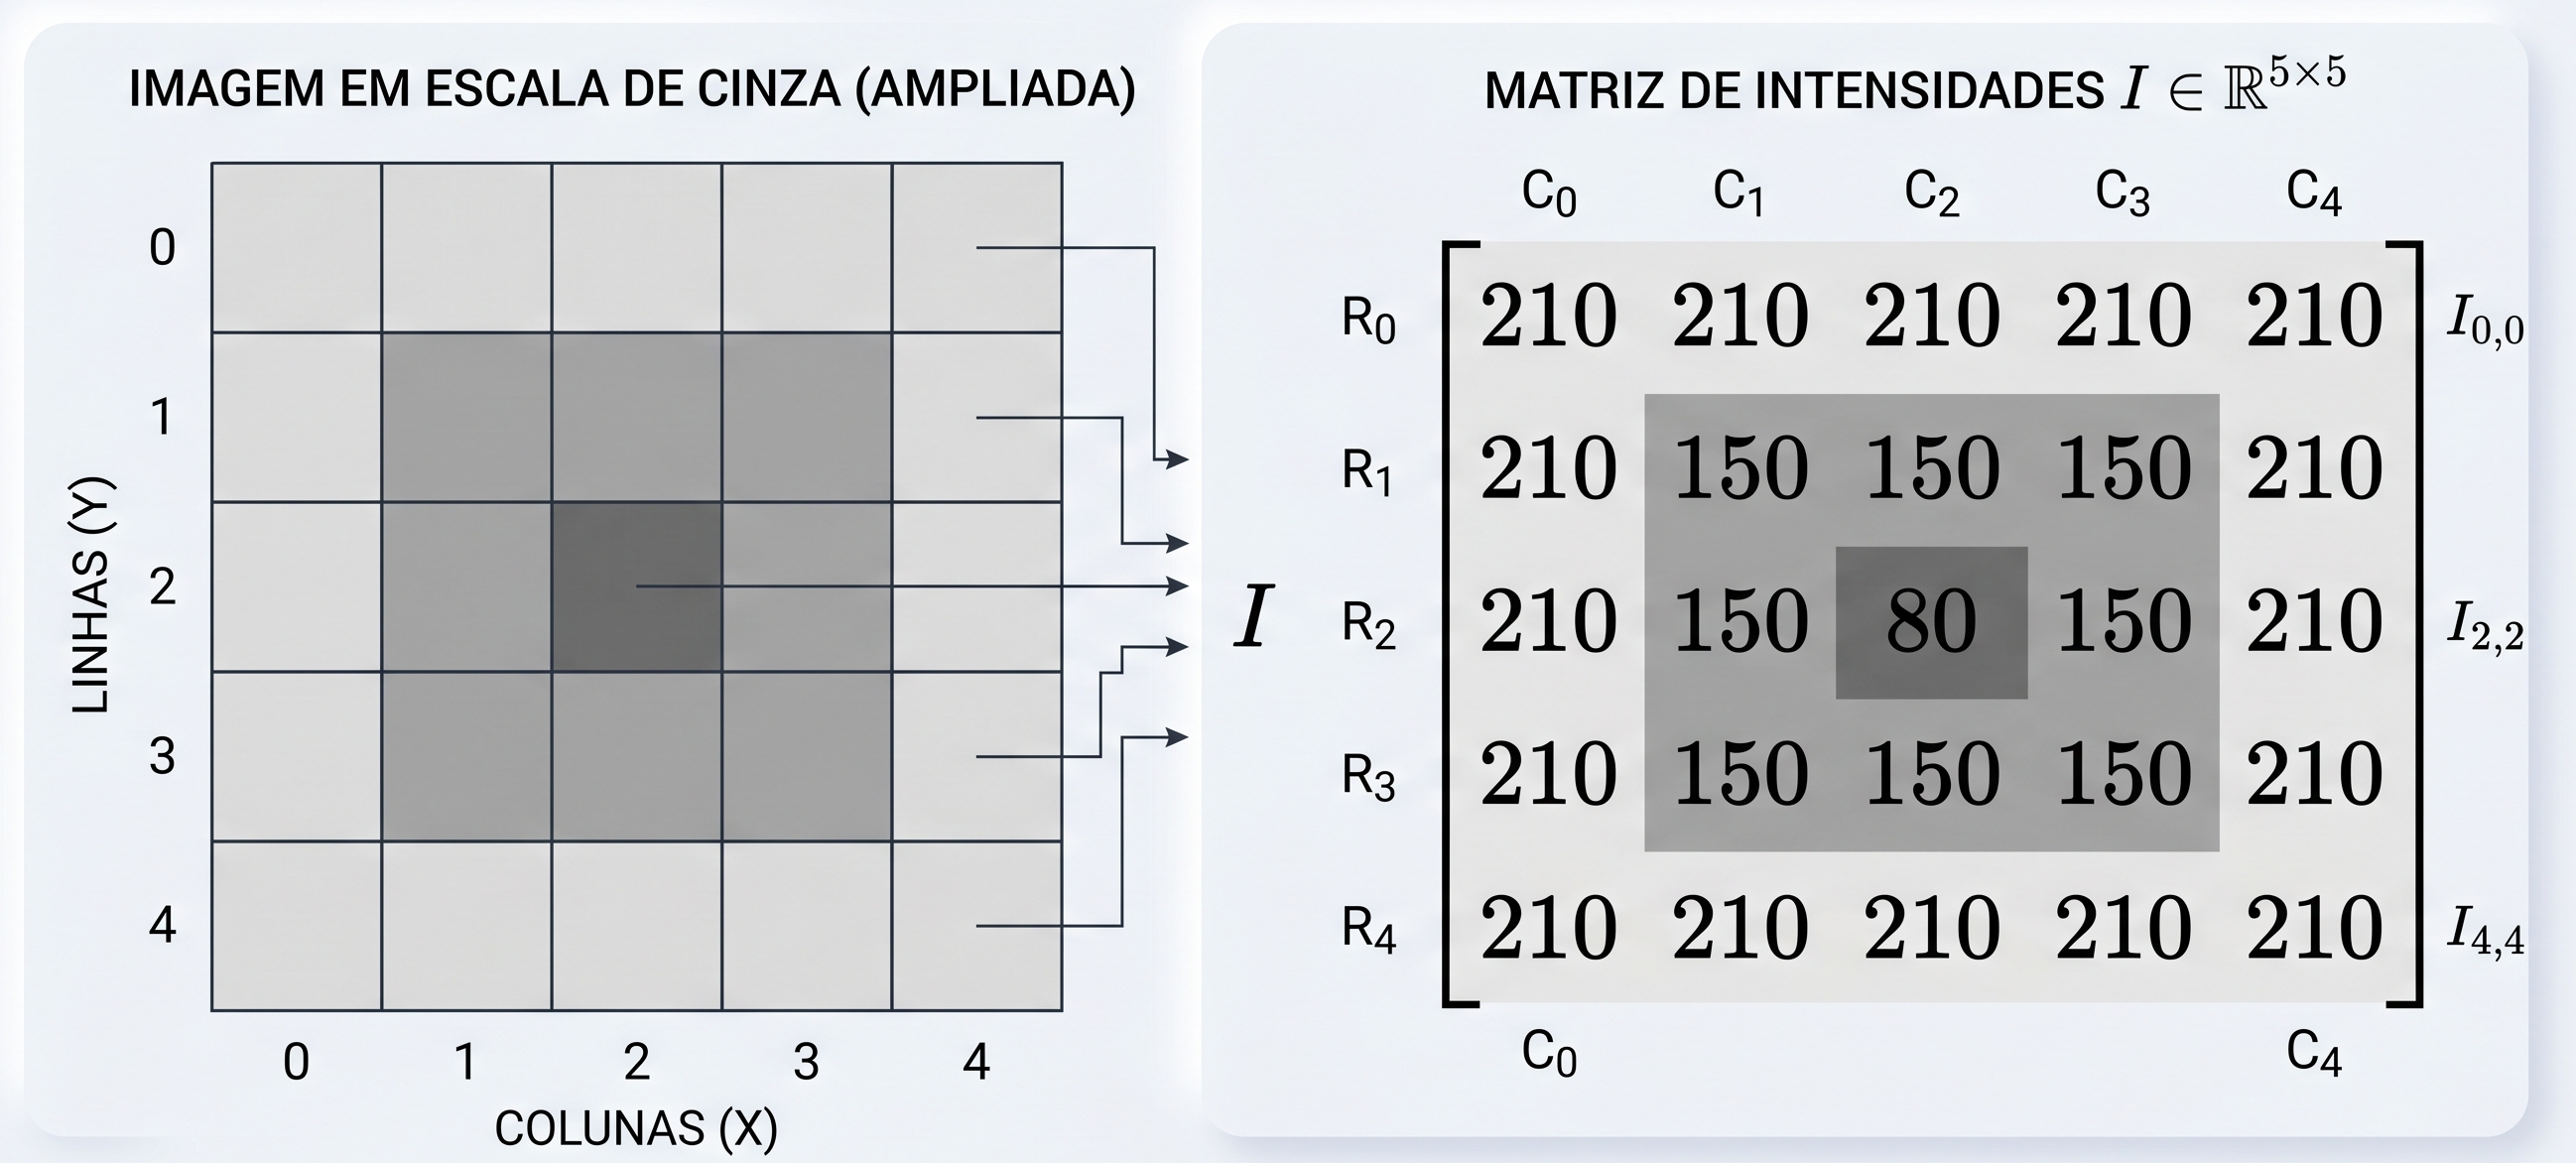
\includegraphics[width=0.78\textwidth]{imagem_matriz_5x5.png}
  \begin{itemize}\small
    \item Imagem em cinza: matriz de pixels; imagem RGB: tensor com 3 canais
    \item As 9 bases variam em resolução (28$\times$28 a 48$\times$48) e canais (1 ou 3)
  \end{itemize}
  \fonte{TCC, Seção 2.4.1 (Representação computacional de imagens digitais).}
\end{frame}

% 8 - Métricas (1:15)
\begin{frame}{Métricas: por que o Macro-F1?}
  \centering
  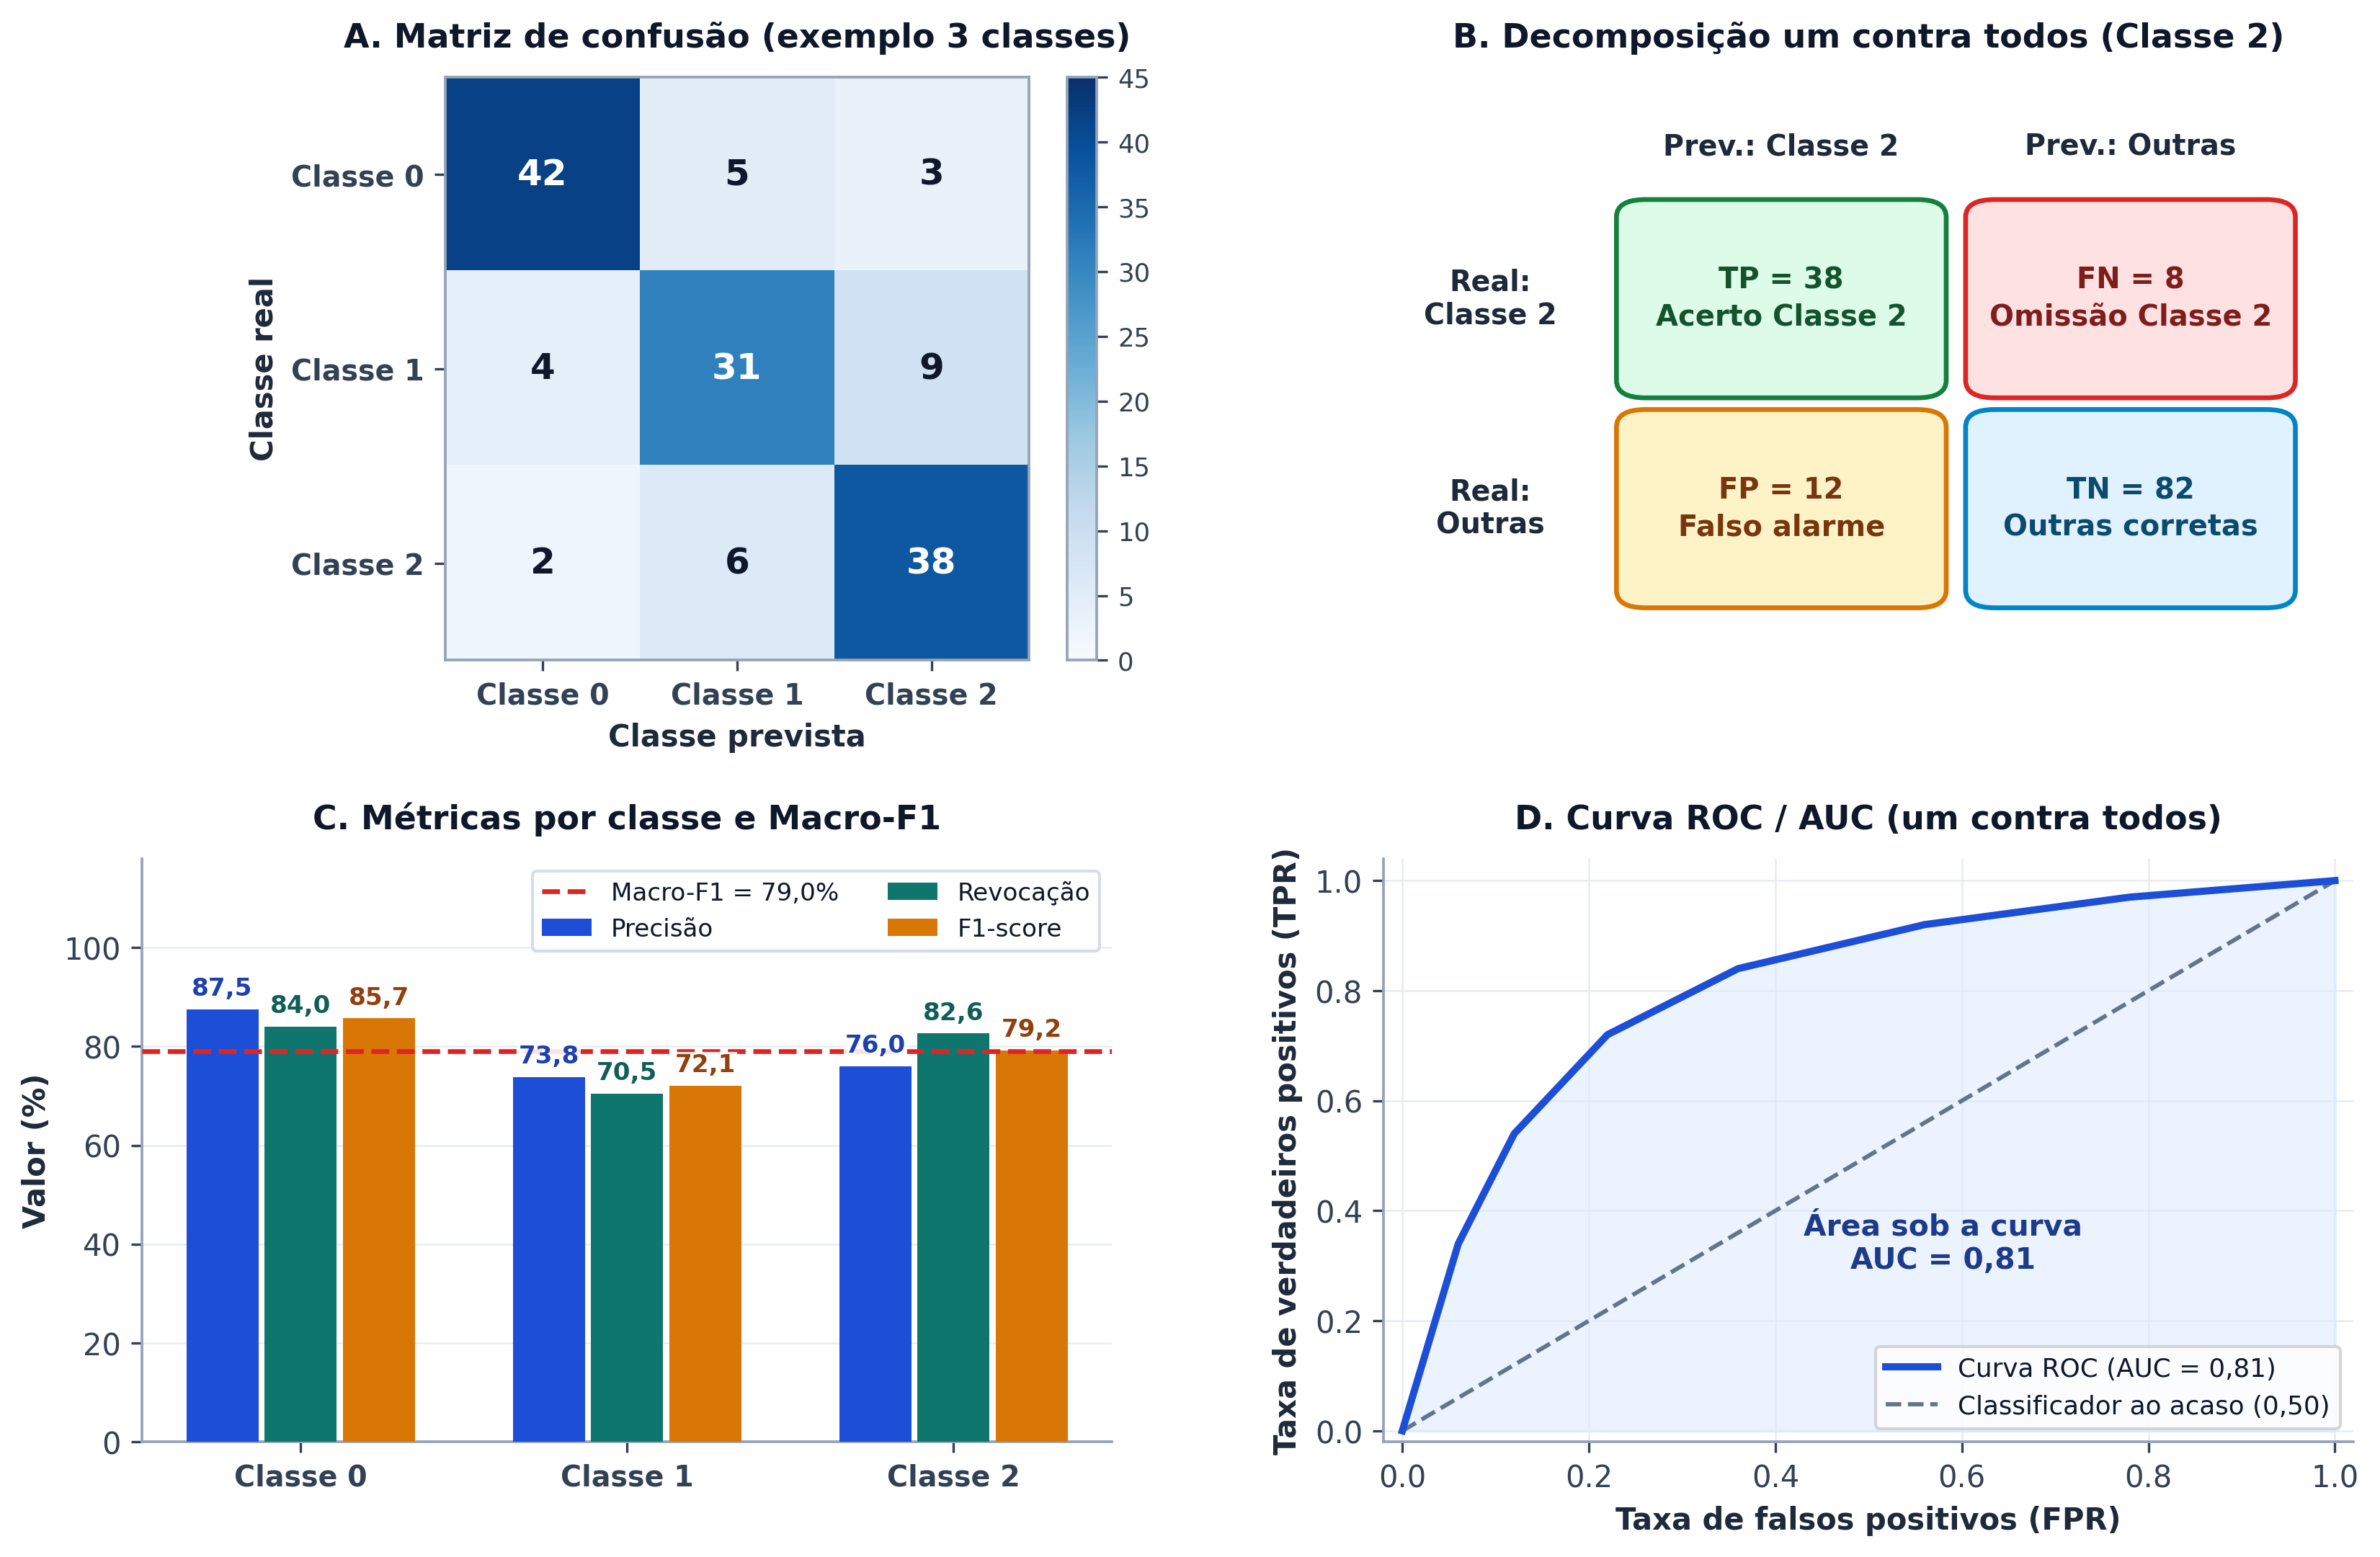
\includegraphics[width=0.66\textwidth]{metricas_classificacao_exemplos.png}
  \begin{itemize}\small
    \item Matriz de confusão, TP/FP/FN/TN por classe (um contra todos), ROC/AUC
    \item \textbf{Macro-F1} = média não ponderada do F1 de todas as classes: dá o mesmo peso às minoritárias (SVHN, GTSRB, FER2013)
  \end{itemize}
  \fonte{TCC, Seção 2.4.4 (Métricas de avaliação).}
\end{frame}

% 9 - Convolução e pooling (1:00)
\begin{frame}{CNN: convolução e \textit{pooling}}
  \centering
  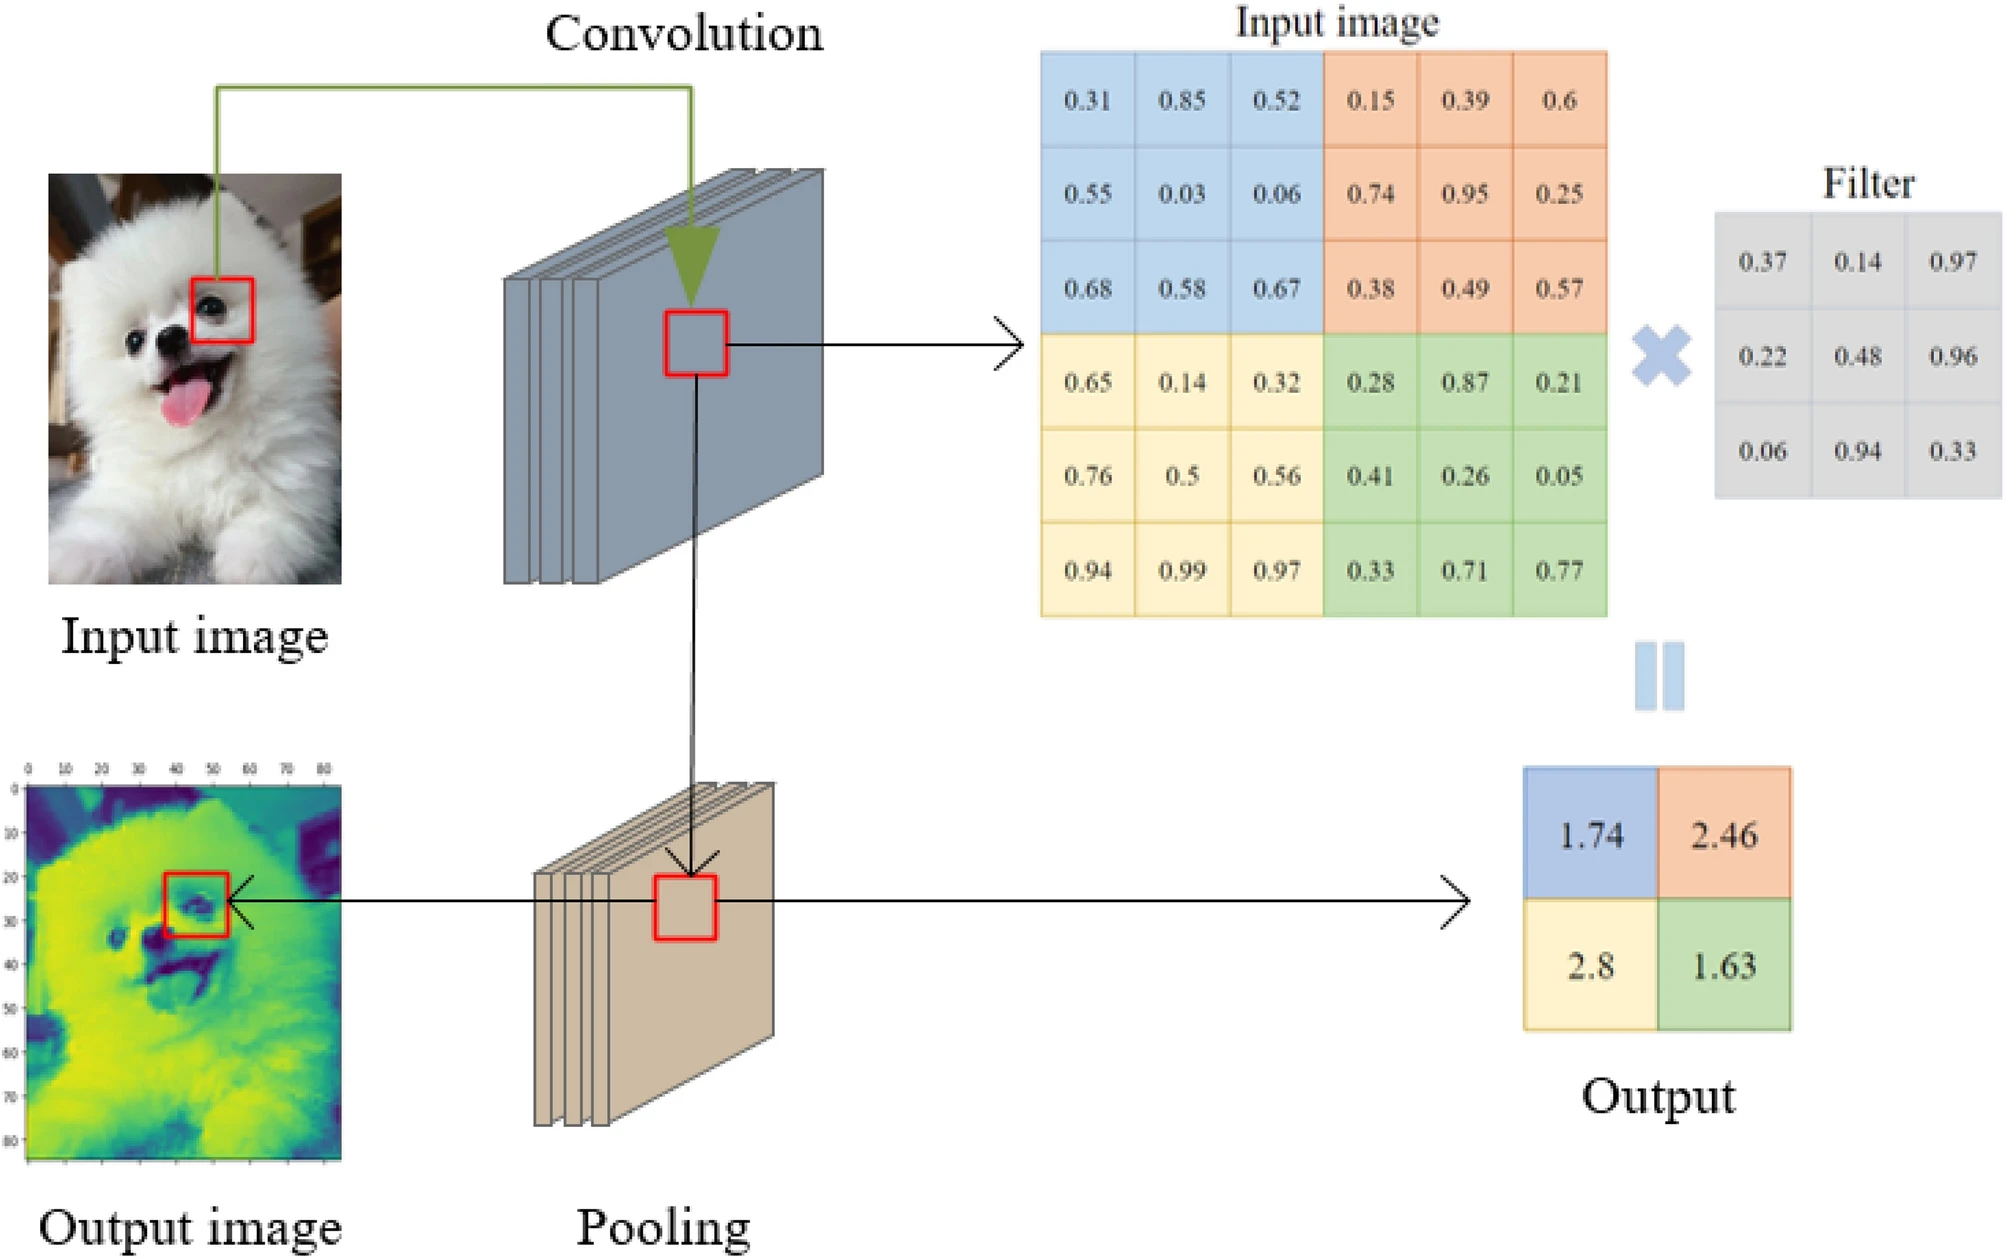
\includegraphics[width=0.62\textwidth]{convolutional-pooling.png}
  \begin{itemize}\small
    \item Filtros treináveis percorrem a imagem e detectam padrões locais
    \item \textit{Pooling} reduz a resolução espacial, mantendo o essencial
  \end{itemize}
  \fonte{TCC, Seção 2.5.2 (Redes neurais convolucionais).}
\end{frame}

% 10 - Mapas de características (0:45)
\begin{frame}{Mapas de características}
  \begin{columns}[c]
    \begin{column}{0.46\textwidth}
      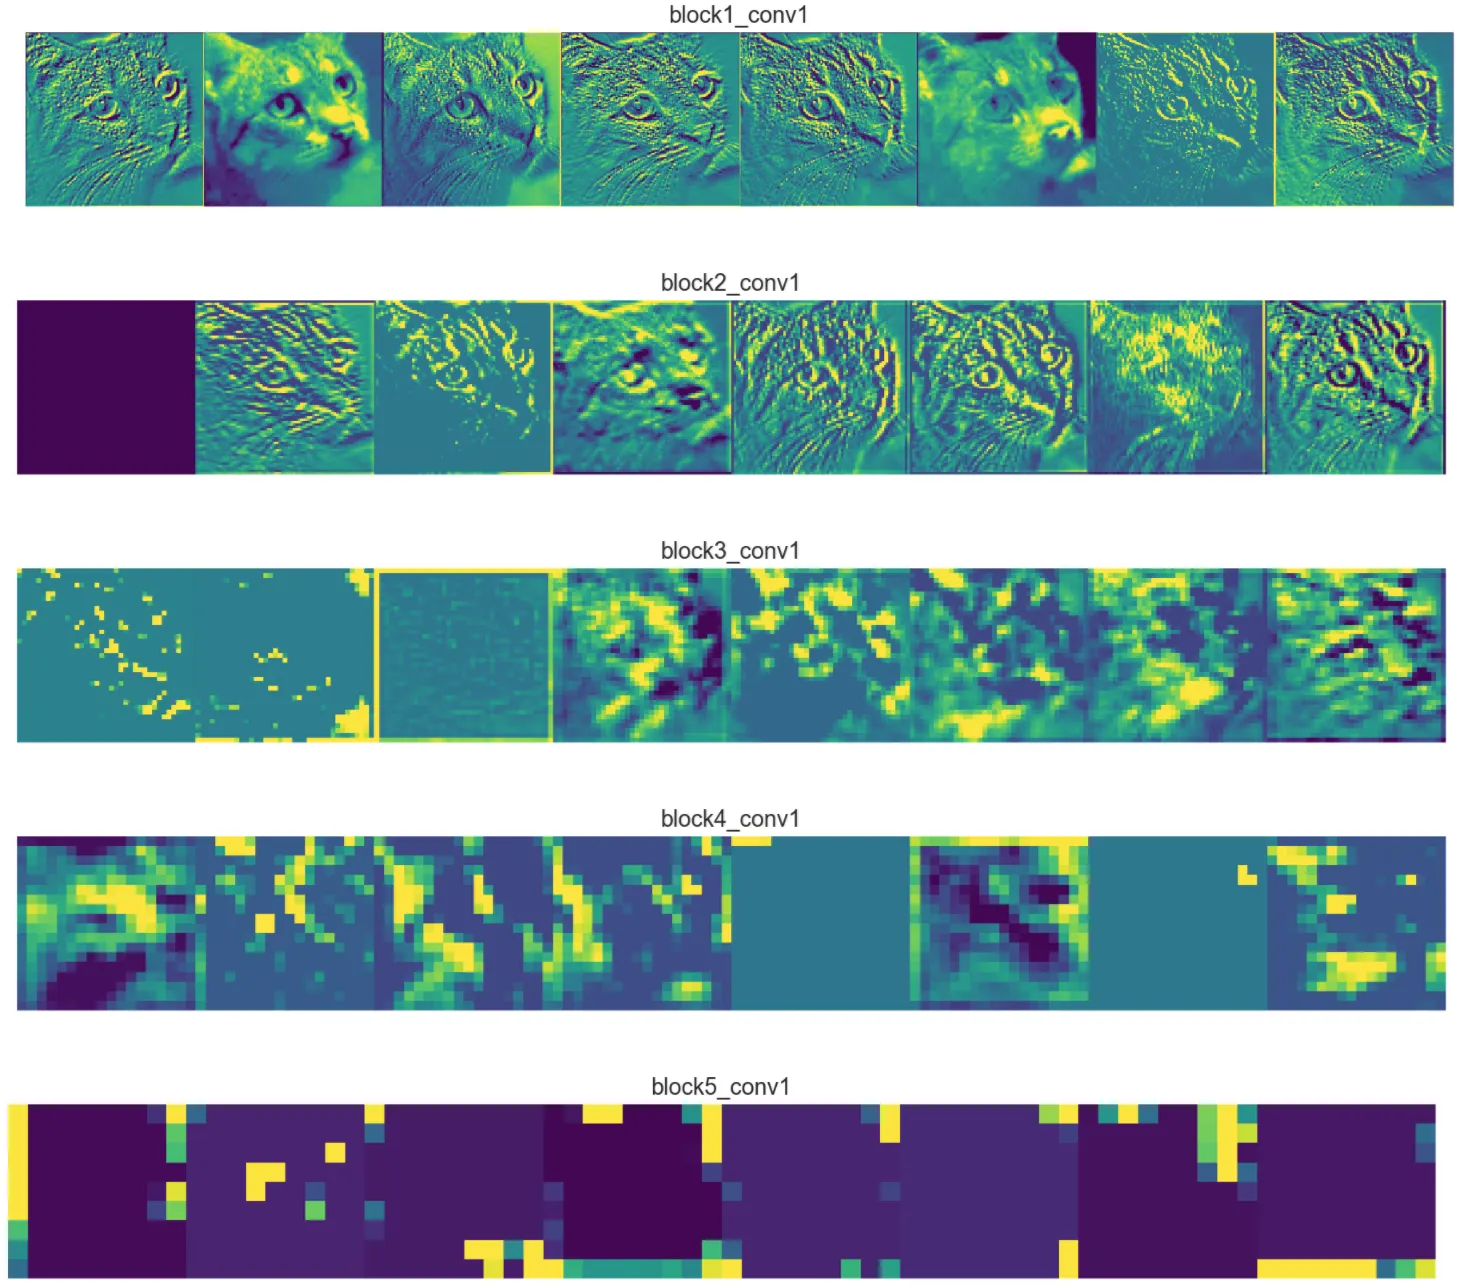
\includegraphics[width=\textwidth]{feature-map-converted.png}
    \end{column}
    \begin{column}{0.48\textwidth}
      \begin{itemize}
        \item Camadas iniciais: bordas, texturas e contornos
        \item Camadas profundas: padrões mais abstratos
        \item O vetor final é o que alimenta a cabeça (densa ou quântica)
      \end{itemize}
    \end{column}
  \end{columns}
  \fonte{TCC, Seção 2.5.2.}
\end{frame}

% 11 - Aumento de dados (0:45)
\begin{frame}{Aumento de dados e \textit{overfitting}}
  \centering
  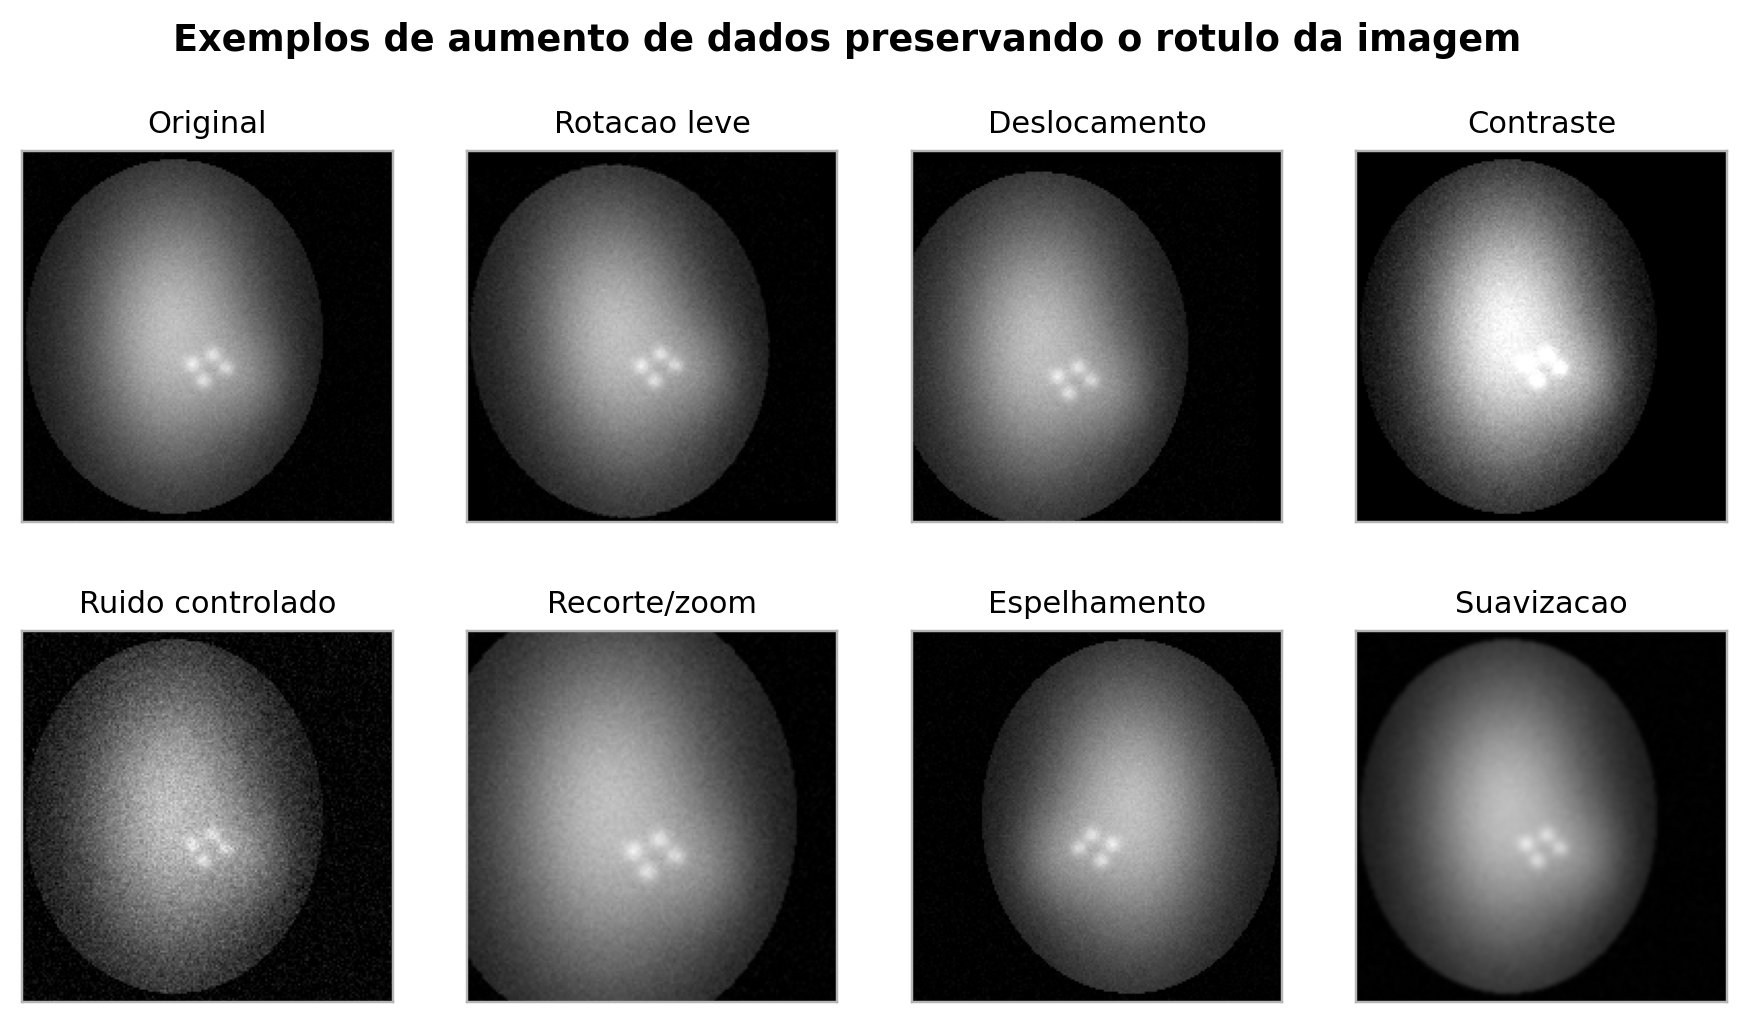
\includegraphics[width=0.66\textwidth]{aumento_dados_exemplos.png}
  \begin{itemize}\small
    \item Transformações leves que preservam o rótulo ampliam a diversidade do treino
    \item Reduz o risco de \textit{overfitting} (ex.: CIFAR-10 em CNN simples: 94\% treino vs. 73\% teste)
  \end{itemize}
  \fonte{TCC, Seção 2.5.4 (Aumento de dados, regularização e \textit{overfitting}); exemplo de CIFAR-10 em Khanday et al. (2021).}
\end{frame}

% 12 - Qubits e circuitos (1:00)
\begin{frame}{Qubits, portas e circuitos quânticos}
  \centering
  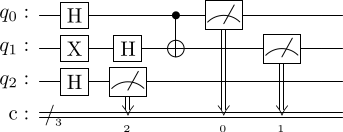
\includegraphics[width=0.55\textwidth]{ibm_visualize_circuits_latex.png}
  \vspace{0.2cm}
  \begin{itemize}\small
    \item Qubit: superposição de $|0\rangle$ e $|1\rangle$; portas $H$, $X$, CNOT criam e transformam estados e emaranhamento
    \item A medição colapsa o estado e devolve valores clássicos
  \end{itemize}
  \fonte{TCC, Seção 2.6.1--2.6.2. Figura ilustrativa da documentação IBM Quantum/Qiskit.}
\end{frame}

% 13 - Codificação + ansatz (1:15)
\begin{frame}{Codificação de dados e \textit{ansatz} parametrizado}
  \centering
  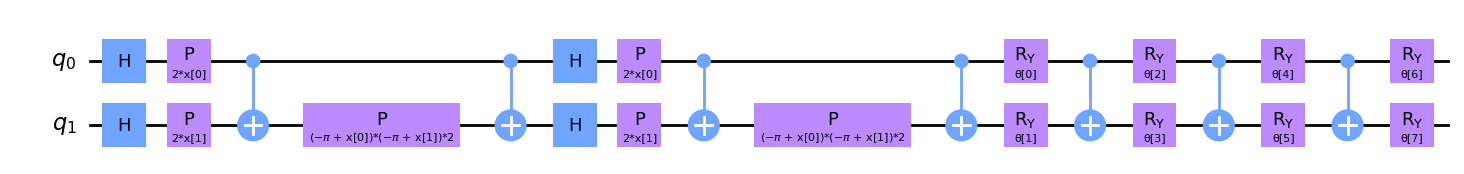
\includegraphics[width=0.95\textwidth]{qiskit_ml_torch_connector_qnn_circuit.png}

  \vspace{0.1cm}
  \begin{columns}[c]
    \begin{column}{0.42\textwidth}
      \centering
      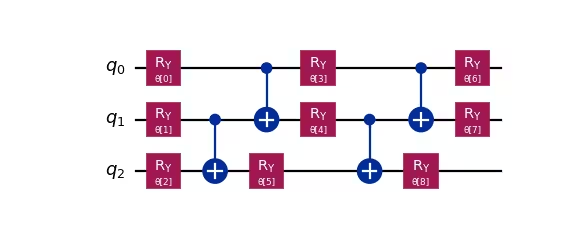
\includegraphics[width=\textwidth]{ibm_real_amplitudes_1.png}
    \end{column}
    \begin{column}{0.54\textwidth}
      \begin{itemize}\small
        \item \textit{Feature map}: dado clássico $\to$ rotações dos qubits
        \item \textit{Ansatz}: camadas $R_Y$ treináveis + CNOT (aqui: \textit{RealAmplitudes})
        \item Parâmetros otimizados por gradiente, como em uma camada neural
      \end{itemize}
    \end{column}
  \end{columns}
  \fonte{TCC, Seções 2.6.3--2.6.4. Figuras ilustrativas da documentação Qiskit; o experimento foi implementado em PennyLane.}
\end{frame}

% 14 - Simulação e limites (1:15)
\begin{frame}{Simulação, \textit{barren plateaus} e escalabilidade}
  \centering
  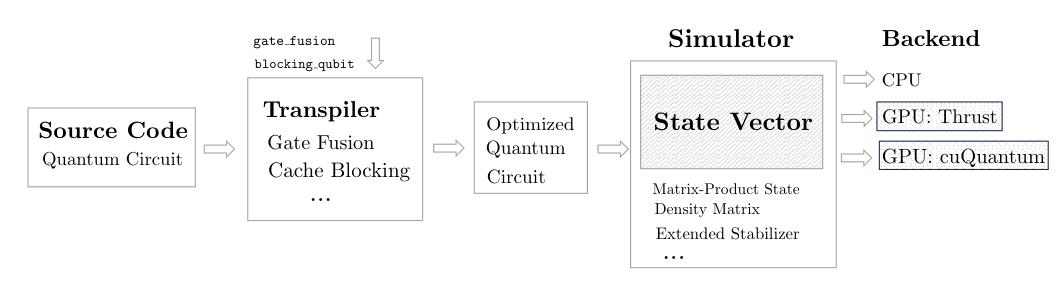
\includegraphics[width=0.92\textwidth]{qiskit_aer_cuquantum_workflow_faj2023.png}
  \begin{itemize}\small
    \item Simular $n$ qubits exige $2^n$ amplitudes: 20 qubits $\Rightarrow$ $2^{20}$ estados por amostra do lote
    \item \textit{Barren plateaus} dificultam o treino de circuitos largos
    \item Consequência de projeto: dividir o circuito (4 $\times$ 5 qubits, $2^5 = 32$ estados cada)
  \end{itemize}
  \fonte{TCC, Seções 2.6.5--2.6.6. Fluxo de simulação do Qiskit Aer (Faj et al., 2023).}
\end{frame}

% ===============================================================
\section{Trabalhos correlatos e lacuna}
% ===============================================================

% 15 - Metodologia da revisão (1:00)
\begin{frame}{Como foi a revisão da literatura}
  \begin{columns}[c]
    \begin{column}{0.55\textwidth}
      \centering
      \begin{tikzpicture}[font=\scriptsize,align=center]
        \node[draw=senacblue,fill=senacblue!15,minimum width=6.4cm,minimum height=0.8cm] (a) {\textbf{5.925} ocorrências brutas (2021--2026)};
        \node[draw=senacblue,fill=senacblue!25,minimum width=5.4cm,minimum height=0.8cm,below=0.15cm of a] (b) {\textbf{3.297} grupos após desduplicação};
        \node[draw=senacblue,fill=senacblue!40,minimum width=4.4cm,minimum height=0.8cm,below=0.15cm of b] (c) {\textbf{1.025} candidatos (triagem automática)};
        \node[draw=senacorange,fill=senacorange!30,minimum width=3.4cm,minimum height=0.8cm,below=0.15cm of c] (d) {\textbf{28} registros verificados\\(19 clássicos + 9 quânticos)};
      \end{tikzpicture}
    \end{column}
    \begin{column}{0.43\textwidth}
      \begin{itemize}\small
        \item Frente 1: fundamentação teórica e artigos originais das bases
        \item Frente 2: estudos empíricos por base
        \item Conferência manual da fonte primária: variante, nº de classes, partição, métrica
        \item Contagens são de mapeamento \textit{preliminar}, não total de elegíveis
      \end{itemize}
    \end{column}
  \end{columns}
  \fonte{TCC, Seção 2.1 (fluxo de busca, triagem e extração).}
\end{frame}

% 16 - Correlatos clássicos (1:00)
\begin{frame}{Estudos clássicos nas 9 bases}
  \centering
  \scriptsize
  \begin{tabular}{@{}lp{4.9cm}r@{}}
    \toprule
    \textbf{Base} & \textbf{Estudo e arquitetura} & \textbf{Resultado} \\
    \midrule
    MNIST & Kabir et al. (2023), VGG-5 + Spinal FC & 99,69\% \\
    Fashion-MNIST & Khanday et al. (2021), CNN rasa & 92,68\% \\
    KMNIST & Kabir et al. (2023) & 99,05\% \\
    EMNIST Balanced & Kabir et al. (2023) & 90,73\% \\
    CIFAR-10 & Khanday et al. (2021) & 73,04\% \\
    CIFAR-100 Coarse & Guo et al. (2018), CNN-RNN, tarefa conjunta & 88,23\% \\
    SVHN & Huang et al. (2017), DenseNet (usa conjunto extra) & 98,41\% \\
    GTSRB & An et al. (2024), LeNet-5 modificada & 97,53\% \\
    FER2013 & Li et al. (2021), Auto-FERNet & 73,78\% \\
    \bottomrule
  \end{tabular}

  \vspace{0.2cm}
  \footnotesize Acurácia de teste reportada pelos autores: \textbf{não equivale} ao Macro-F1 deste trabalho; protocolos e partições diferem.
  \fonte{TCC, Tabela de correlatos clássicos (Seção 2.8.1).}
\end{frame}

% 17 - Correlatos quânticos (1:15)
\begin{frame}{Estudos quânticos e híbridos}
  \begin{columns}[T]
    \begin{column}{0.60\textwidth}
      \scriptsize
      \begin{tabular}{@{}R{2.2cm}R{4.6cm}@{}}
        \toprule
        \textbf{Base} & \textbf{Recorte e resultado} \\
        \midrule
        MNIST & 3 vs. 5 binário: 98,85\% (Long, 2025); NNQE 10 classes: 93,8\% (Riaz, 2023) \\
        Fashion-MNIST & 4 classes: 85,93\% vs. 89,69\% clássico (Bokhan, 2022) \\
        KMNIST & Apenas binário (Dong, 2025) \\
        EMNIST & 75,9\% com filtro quântico fixo (Riaz, 2026) \\
        CIFAR-10 & NNQE: 36,0\% (Riaz, 2023) \\
        \textbf{CIFAR-100 Coarse} & \textbf{Nenhum estudo identificado} \\
        GTSRB & NNQE \textbf{73,4\%} vs. \textbf{82,2\%} clássico \\
        \bottomrule
      \end{tabular}
    \end{column}
    \begin{column}{0.37\textwidth}
      \begin{itemize}\small
        \item Recortes binários, 4 classes ou conjuntos sintéticos
        \item Filtros quânticos fixos seguidos de camadas densas
        \item O NNQE no GTSRB mostra: híbrido \textit{não} melhora todas as tarefas
      \end{itemize}
    \end{column}
  \end{columns}
  \fonte{TCC, Tabela de correlatos quânticos/híbridos (Seção 2.8.2).}
\end{frame}

% 18 - Lacuna (0:45)
\begin{frame}{Lacuna de pesquisa}
  \begin{enumerate}
    \item \textbf{Protocolos fragmentados:} poucas classes, poucos domínios; nenhum resultado quântico para as 20 superclasses do CIFAR-100 Coarse
    \item \textbf{Só acurácia:} Macro-F1 raramente reportado, justamente onde há desbalanceamento (GTSRB, FER2013, SVHN)
    \item \textbf{Variáveis de confusão:} lotes diferentes, ausência de controle clássico com gargalo equivalente
  \end{enumerate}
  \vspace{0.3cm}
  \begin{block}{Contribuição proposta}
    Campanha padronizada nas 9 bases completas, avaliada por Macro-F1 e com controle vetorial de gargalo (\texttt{Dense20}).
  \end{block}
\end{frame}

% ===============================================================
\section{Desenvolvimento}
% ===============================================================

% 19 - Tipo de pesquisa e pergunta (0:45)
\begin{frame}{Tipo de pesquisa e pergunta de pesquisa}
  \begin{itemize}
    \item \textbf{Aplicada}, abordagem \textbf{quantitativa}
    \item Objetivos \textbf{exploratórios} (CIFAR-100 Coarse e EMNIST pouco explorados em QML), \textbf{descritivos} (72 \textit{checkpoints} documentados) e \textbf{comparativos}
  \end{itemize}
  \begin{block}{Pergunta de pesquisa}
    Nas nove bases, como se comporta o Macro-F1 do híbrido (4 circuitos de 5 qubits) frente à CNN original e ao controle \texttt{Dense20}, sob as mesmas partições, e que limites de generalização e custo emergem?
  \end{block}
\end{frame}

% 20 - Pipeline (0:45)
\begin{frame}{Pipeline experimental em seis etapas}
  \centering
  \begin{tikzpicture}[node distance=0.5cm and 0.7cm,
      box/.style={draw=senacblue,rounded corners,fill=senacblue!8,font=\scriptsize,align=center,minimum height=0.9cm,text width=3.3cm},
      arr/.style={-{Stealth},thick,senacblue}]
    \node[box] (e1) {\textbf{1. Inventário}\\9 bases padronizadas};
    \node[box,right=of e1] (e2) {\textbf{2. Pré-processamento}\\normalização, 64$\times$64, partição estratificada};
    \node[box,right=of e2] (e3) {\textbf{3. CNN clássica}\\baseline e variações};
    \node[box,below=of e1] (e4) {\textbf{4. Controle \texttt{Dense20}}\\gargalo vetorial de 20 dim.};
    \node[box,right=of e4] (e5) {\textbf{5. Híbrido}\\4 circuitos $\times$ 5 qubits, treino fim a fim};
    \node[box,right=of e5] (e6) {\textbf{6. Auditoria}\\Macro-F1, matrizes, $\Delta$F1, Grad-CAM};
    \draw[arr] (e1) -- (e2); \draw[arr] (e2) -- (e3);
    \draw[arr] (e3.south) -- ++(0,-0.25) -| ($(e4.north)+(0,0.25)$) -- (e4.north);
    \draw[arr] (e4) -- (e5); \draw[arr] (e5) -- (e6);
  \end{tikzpicture}
  \fonte{TCC, Seção 3.3 (Visão geral da solução proposta).}
\end{frame}

% 21 - As 9 bases (1:15)
\begin{frame}{As nove bases de dados}
  \centering
  \scriptsize
  \begin{tabular}{@{}llcrr@{}}
    \toprule
    \textbf{Base} & \textbf{Domínio} & \textbf{Entrada original} & \textbf{Classes} & \textbf{Treino / Val. / Teste} \\
    \midrule
    MNIST & dígitos manuscritos & 28$\times$28, cinza & 10 & 48.999 / 10.503 / 10.498 \\
    Fashion-MNIST & vestuário & 28$\times$28, cinza & 10 & 49.000 / 10.500 / 10.500 \\
    KMNIST & caracteres Kuzushiji & 28$\times$28, cinza & 10 & 49.000 / 10.500 / 10.500 \\
    EMNIST Balanced & alfanumérico & 28$\times$28, cinza & \textbf{47} & 92.120 / 19.740 / 19.740 \\
    CIFAR-10 & objetos e animais & 32$\times$32, RGB & 10 & 42.000 / 9.000 / 9.000 \\
    CIFAR-100 Coarse & superclasses & 32$\times$32, RGB & \textbf{20} & 42.000 / 9.000 / 9.000 \\
    SVHN & dígitos de fachadas & 32$\times$32, RGB & 10 & 69.502 / 14.894 / 14.893 \\
    GTSRB & placas de trânsito & variável, RGB & \textbf{43} & 27.489 / 5.905 / 5.876 \\
    FER2013 & expressões faciais & 48$\times$48, cinza & 7 & 25.121 / 5.384 / 5.382 \\
    \bottomrule
  \end{tabular}

  \vspace{0.2cm}
  \footnotesize Partições da campanha auditada (30/10/2026), não as divisões oficiais.
  \fonte{TCC, Tabela de caracterização dos 9 conjuntos de dados (Seção 2.3.2).}
\end{frame}

% 22 - Desbalanceamento (1:15)
\begin{frame}{Equilíbrio de classes: três regimes}
  \begin{columns}[c]
    \begin{column}{0.68\textwidth}
      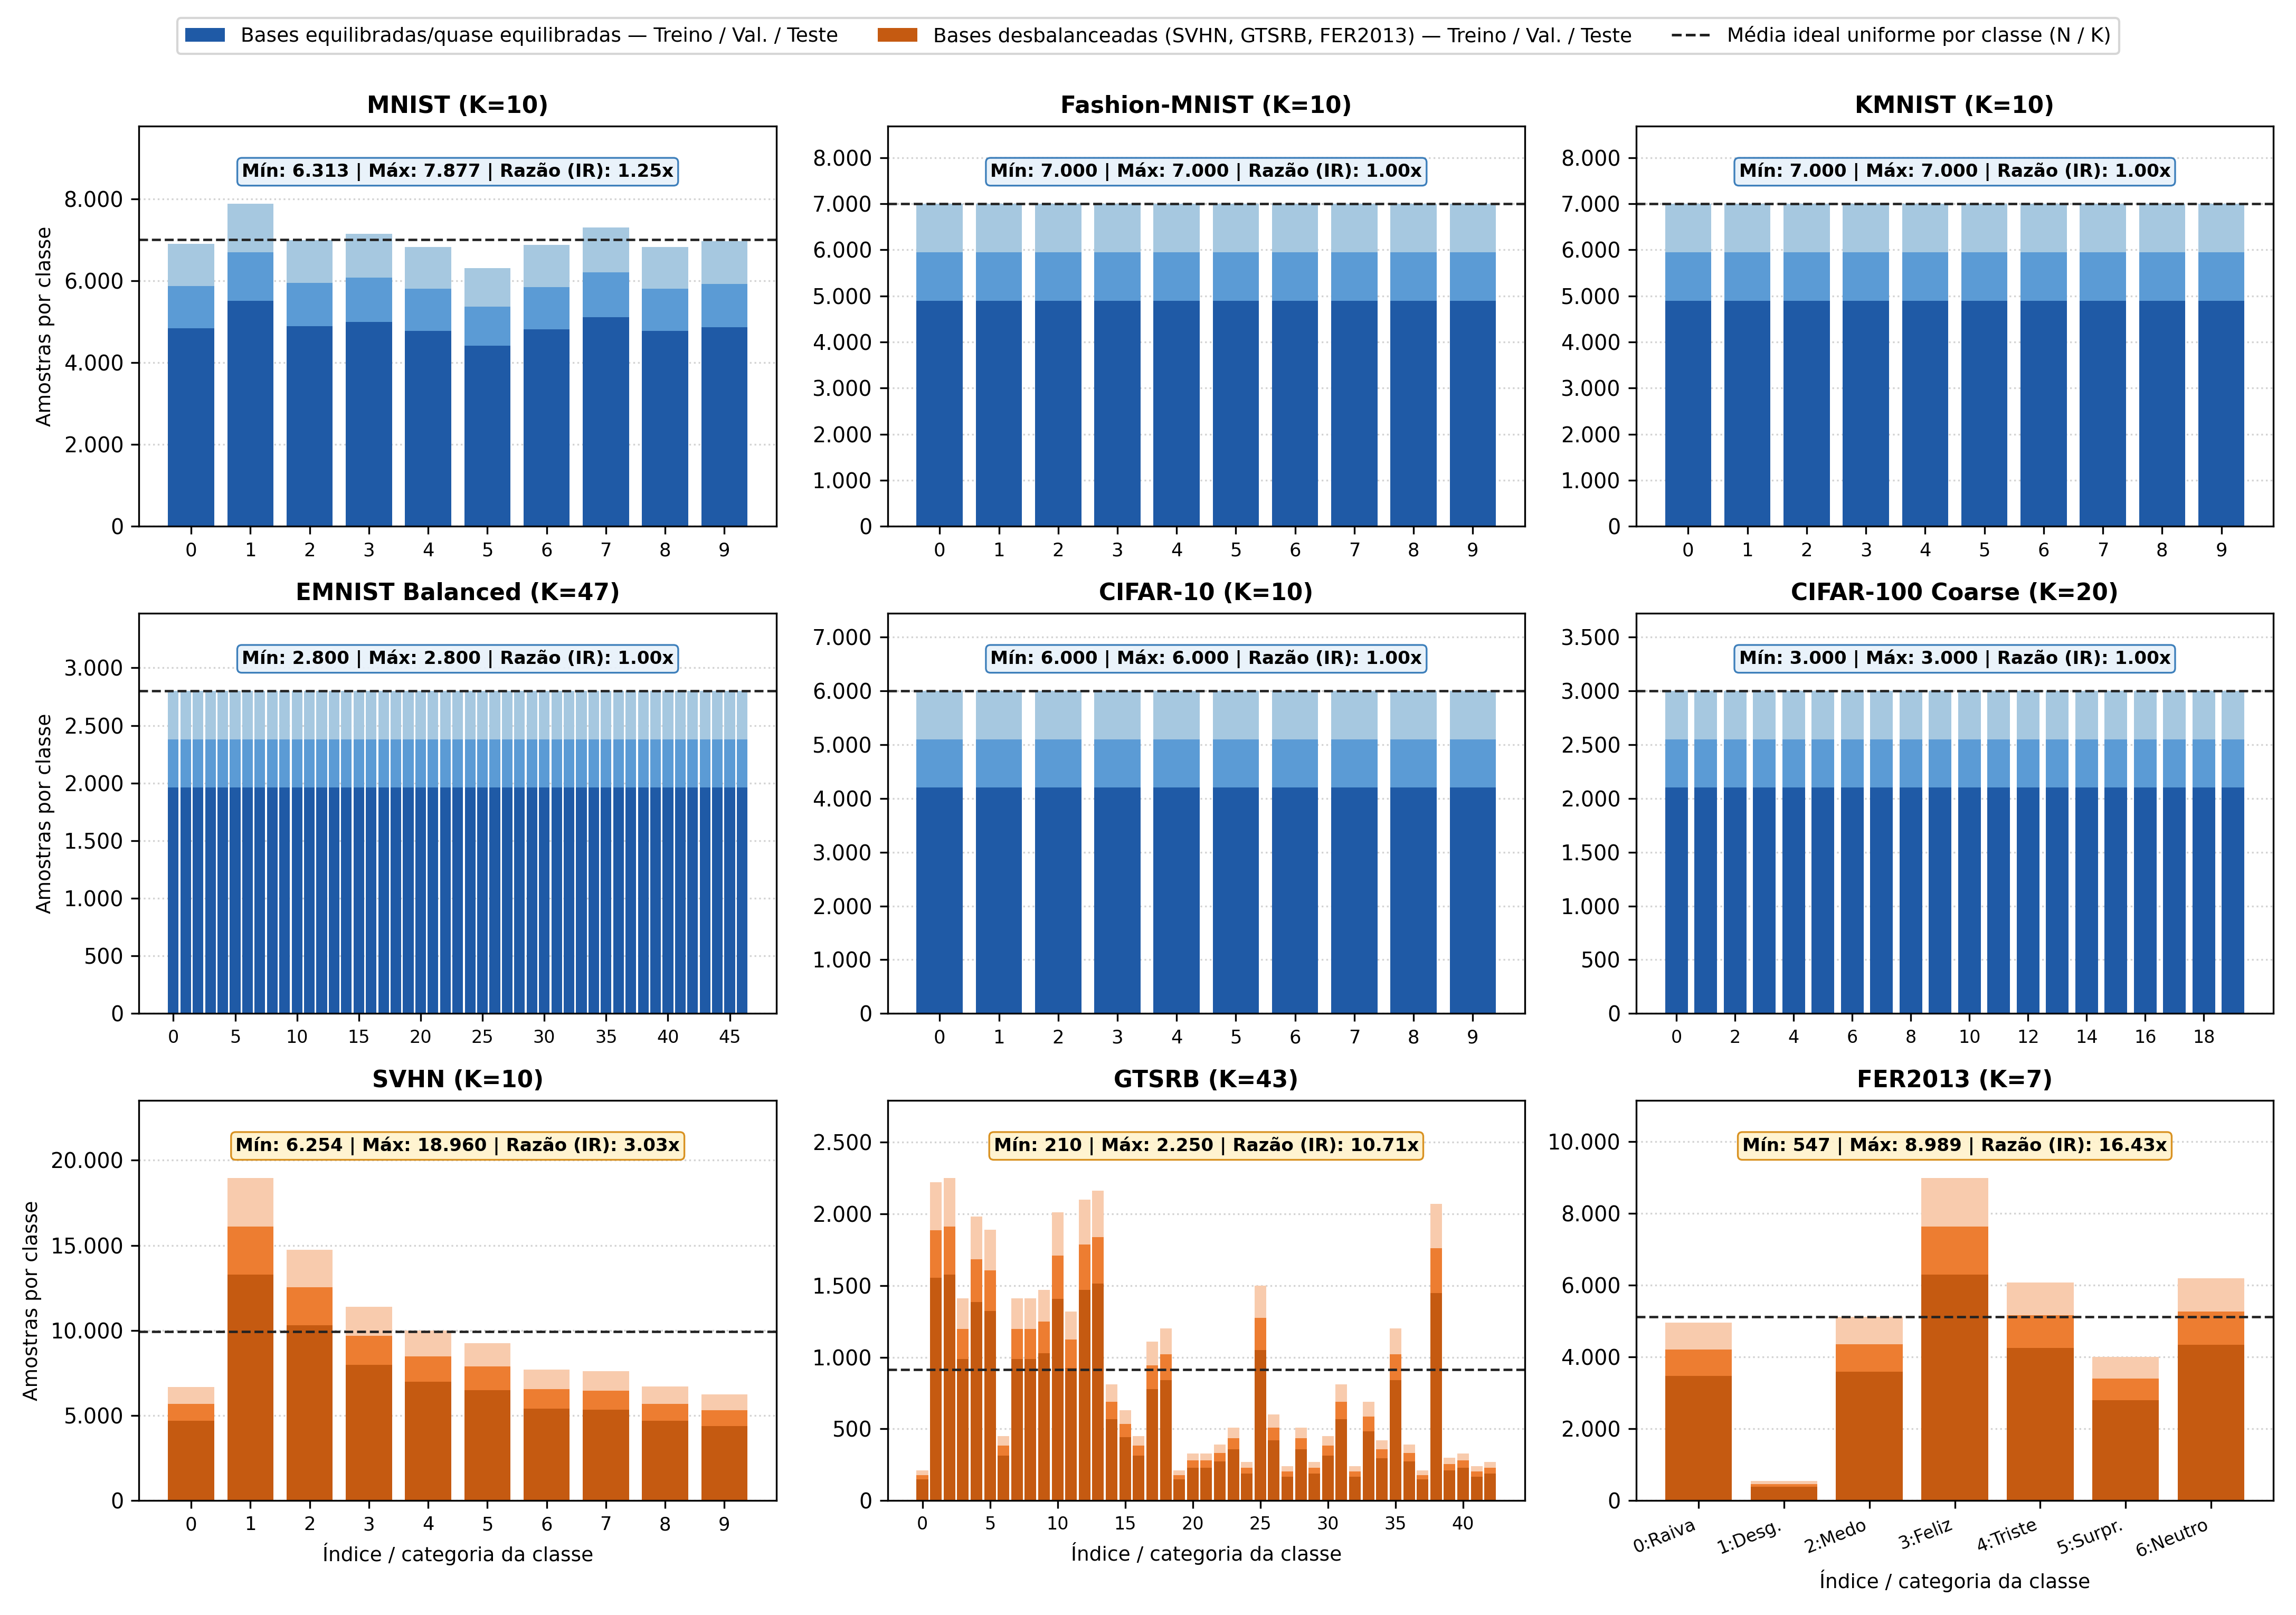
\includegraphics[width=\textwidth]{equilibrio_classes_9_datasets.png}
    \end{column}
    \begin{column}{0.30\textwidth}
      \footnotesize
      \begin{itemize}
        \item \textbf{IR = 1,00$\times$:} Fashion-MNIST, KMNIST, EMNIST, CIFAR-10, CIFAR-100 Coarse
        \item \textbf{IR = 1,25$\times$:} MNIST
        \item \textbf{IR = 3,03 a 16,43$\times$:} SVHN, GTSRB (10,71$\times$) e FER2013 (16,43$\times$; só 547 imagens de ``desgosto'')
      \end{itemize}
      \footnotesize IR = $n_{\max}/n_{\min}$. Validação e teste mantêm a distribuição original.
    \end{column}
  \end{columns}
  \fonte{TCC, Figura de distribuição de amostras por classe (Seção 2.3.3).}
\end{frame}

% 23 - Pré-processamento + ressalva GTSRB (1:00)
\begin{frame}{Pré-processamento e ressalva do GTSRB}
  \begin{columns}[T]
    \begin{column}{0.48\textwidth}
      \textbf{Idêntico entre modelos de cada base}
      \begin{itemize}
        \item Tensores em ponto flutuante, normalização por canal
        \item Redimensionamento: 64$\times$64 (128$\times$128 no GTSRB)
        \item Partição estratificada, fixa para os 8 modelos de cada base
      \end{itemize}
    \end{column}
    \begin{column}{0.48\textwidth}
      \begin{alertblock}{Limitação auditada: GTSRB}
        \textbf{3.990 das 5.876} imagens de teste compartilham a mesma sequência física (\textit{track}) com imagens de treino.\\[2pt]
        Resultados não são o teste oficial; exigem divisão \textit{track-aware} em trabalhos futuros.
      \end{alertblock}
    \end{column}
  \end{columns}
\end{frame}

% 24 - Três famílias de modelos (1:00)
\begin{frame}{Três famílias de modelos comparadas}
  \begin{columns}[T]
    \begin{column}{0.32\textwidth}
      \begin{block}{CNN original}
        Blocos \texttt{Conv2d}, \texttt{BatchNorm2d}, ativação e \textit{pooling}; cabeça direta para os $K$ \textit{logits}.\\[2pt]\footnotesize Base das variações de ativação, lote e quantização.
      \end{block}
    \end{column}
    \begin{column}{0.32\textwidth}
      \begin{block}{CNN + \texttt{Dense20}}
        Projeta as características para um vetor clássico de \textbf{20 dimensões} antes da camada linear.\\[2pt]\footnotesize \textbf{Controle:} isola o efeito do gargalo.
      \end{block}
    \end{column}
    \begin{column}{0.32\textwidth}
      \begin{block}{CNN + híbrido}
        Mesmo gargalo de 20 dim., processado por \textbf{4 circuitos de 5 qubits} (PennyLane) e camada linear final.\\[2pt]\footnotesize Treino fim a fim.
      \end{block}
    \end{column}
  \end{columns}
  \vspace{0.3cm}
  \centering\small Total: \textbf{72 \textit{checkpoints}} = 9 bases $\times$ 8 configurações
\end{frame}

% 25 - Cabeça híbrida (1:30)
\begin{frame}{Cabeça híbrida: 4 circuitos independentes de 5 qubits}
  \centering
  \begin{tikzpicture}[node distance=0.35cm,
      box/.style={draw=senacblue,rounded corners,fill=senacblue!8,font=\scriptsize,align=center,minimum height=0.9cm},
      q/.style={draw=senacorange,rounded corners,fill=senacorange!15,font=\scriptsize,align=center,minimum height=0.55cm,minimum width=2.3cm},
      arr/.style={-{Stealth},thick,senacblue}]
    \node[box] (img) {Imagem};
    \node[box,right=0.45cm of img] (cnn) {CNN\\(extrator)};
    \node[box,right=0.45cm of cnn] (proj) {Projeção\\$u\in\mathbb{R}^{20}$};
    \node[q,right=1.1cm of proj,yshift=1.05cm] (c1) {Circuito 1 (5 qubits)\\$u^{(1)}\in\mathbb{R}^5$};
    \node[q,below=0.2cm of c1] (c2) {Circuito 2 (5 qubits)\\$u^{(2)}$};
    \node[q,below=0.2cm of c2] (c3) {Circuito 3 (5 qubits)\\$u^{(3)}$};
    \node[q,below=0.2cm of c3] (c4) {Circuito 4 (5 qubits)\\$u^{(4)}$};
    \node[box] (z) at ($(c2.east)!0.5!(c3.east)+(2.2,0)$) {$\langle Z\rangle$ concatenados\\$z\in[-1,1]^{20}$};
    \node[box,right=0.4cm of z] (out) {Linear\\$K$ classes};
    \draw[arr] (img)--(cnn); \draw[arr] (cnn)--(proj);
    \foreach \c in {c1,c2,c3,c4}{\draw[arr] (proj.east)--(\c.west); \draw[arr] (\c.east)--(z.west);}
    \draw[arr] (z)--(out);
    \node[font=\tiny,below=0.15cm of c4,text width=7cm,align=center,color=gray] {Codificação angular $\to$ ansatz (rotações + emaranhamento interno) $\to$ medição de Pauli-$Z$};
  \end{tikzpicture}

  \vspace{0.1cm}
  \begin{itemize}\small
    \item $4\times5=20$ entradas; cada circuito opera em $2^5=32$ estados (um único de 20 qubits seria intratável)
    \item \textbf{Sem emaranhamento entre os 4 subcircuitos}
  \end{itemize}
  \fonte{TCC, Seção 3.7 (Modelo híbrido quântico-clássico). Diagrama elaborado pelo autor.}
\end{frame}

% 26 - Protocolo (1:00)
\begin{frame}{Protocolo experimental}
  \begin{columns}[T]
    \begin{column}{0.48\textwidth}
      \begin{itemize}
        \item \textbf{72 \textit{checkpoints}} (9 $\times$ 8), campanha auditada de 30/10/2026
        \item \textbf{Uma semente} por configuração; \textit{checkpoint} escolhido pela validação e avaliado no teste
        \item Python, PyTorch, PennyLane; Windows (GPU CUDA) e macOS (Apple Silicon)
      \end{itemize}
    \end{column}
    \begin{column}{0.48\textwidth}
      \begin{block}{Métrica primária}
        Macro-F1 de teste (\%) e $\Delta$ pareado em pontos percentuais
      \end{block}
      \textbf{Critérios:}
      \begin{enumerate}\small
        \item Convergência estável acima do acaso ($1/K$)
        \item Magnitude das diferenças entre os três modelos
        \item Comportamento com mais classes e maior complexidade
      \end{enumerate}
    \end{column}
  \end{columns}
\end{frame}

% ===============================================================
\section{Resultados e discussão}
% ===============================================================

% 27 - Tabela Macro-F1 (1:30)
\begin{frame}{Macro-F1 de teste (\%) nas nove bases}
  \centering
  \footnotesize
  \begin{tabular}{@{}lrrrrr@{}}
    \toprule
    \textbf{Base} & \textbf{CNN orig.} & \textbf{Dense20} & \textbf{Híbrido} & \textbf{$\Delta$ Híb.$-$CNN} & \textbf{$\Delta$ Híb.$-$Dense20} \\
    \midrule
    MNIST & 98,984 & 99,225 & 99,305 & $+0{,}321$ & $+0{,}080$ \\
    Fashion-MNIST & 91,915 & 92,050 & 91,894 & $-0{,}021$ & $-0{,}156$ \\
    KMNIST & 98,649 & 98,648 & 98,648 & $-0{,}001$ & $0{,}000$ \\
    EMNIST Balanced & 87,719 & 88,642 & 88,474 & $+0{,}755$ & $-0{,}168$ \\
    CIFAR-10 & 73,117 & 73,389 & 73,320 & $+0{,}203$ & $-0{,}069$ \\
    CIFAR-100 Coarse & 47,458 & 47,559 & 47,117 & $-0{,}341$ & $-0{,}442$ \\
    SVHN & 92,088 & 92,567 & 92,634 & $+0{,}546$ & $+0{,}067$ \\
    GTSRB* & 99,365 & 99,633 & 99,590 & $+0{,}225$ & $-0{,}043$ \\
    FER2013 & 48,158 & 47,899 & 48,519 & $+0{,}361$ & $+0{,}620$ \\
    \bottomrule
  \end{tabular}

  \vspace{0.15cm}
  \tiny *GTSRB: teste com sobreposição de \textit{tracks} (3.990 de 5.876); não é o teste oficial. Comparação arquitetural centrada em 3 das 8 configurações por base.
  \fonte{TCC, Tabela de resultados próprios (Seção 4.1), campanha de 30/10/2026.}
\end{frame}

% 28 - Gráfico dos deltas (1:15)
\begin{frame}{Quanto o híbrido difere? ($\Delta$ em pontos percentuais)}
  \centering
  \begin{tikzpicture}
    \begin{axis}[
        ybar, width=13.2cm, height=4.9cm, bar width=5pt,
        ymin=-0.6, ymax=0.9, ylabel={$\Delta$ Macro-F1 (p.p.)},
        ylabel style={font=\scriptsize},
        symbolic x coords={MNIST,F-MNIST,KMNIST,EMNIST,CIFAR-10,CIFAR-100C,SVHN,GTSRB,FER2013},
        xtick=data, x tick label style={font=\tiny,rotate=25,anchor=east},
        y tick label style={font=\tiny},
        legend style={font=\tiny,at={(0.5,1.12)},anchor=south,legend columns=2},
        enlarge x limits=0.07, ymajorgrids, grid style={dotted,gray},
        extra y ticks=0, extra y tick style={grid=major,grid style={solid,black}},
      ]
      \addplot[fill=senacblue!80,draw=none] coordinates {(MNIST,0.321)(F-MNIST,-0.021)(KMNIST,-0.001)(EMNIST,0.755)(CIFAR-10,0.203)(CIFAR-100C,-0.341)(SVHN,0.546)(GTSRB,0.225)(FER2013,0.361)};
      \addplot[fill=senacorange,draw=none] coordinates {(MNIST,0.080)(F-MNIST,-0.156)(KMNIST,0.000)(EMNIST,-0.168)(CIFAR-10,-0.069)(CIFAR-100C,-0.442)(SVHN,0.067)(GTSRB,-0.043)(FER2013,0.620)};
      \legend{Híbrido $-$ CNN original, Híbrido $-$ \texttt{Dense20}}
    \end{axis}
  \end{tikzpicture}

  \small Frente à CNN: média $+0{,}23$ p.p.; frente ao \texttt{Dense20}: média $-0{,}01$ p.p. (híbrido melhor em apenas 3 de 9; KMNIST empata).
  \fonte{Elaborado pelo autor a partir da Tabela de resultados do TCC (Seção 4.1); médias calculadas sobre os nove $\Delta$.}
\end{frame}

% 29 - Papel do Dense20 (1:30)
\begin{frame}{O papel do controle \texttt{Dense20}}
  \begin{columns}[T]
    \begin{column}{0.50\textwidth}
      \begin{alertblock}{Sem o controle, haveria ``ganhos''}
        Híbrido $-$ CNN: EMNIST $+0{,}755$, SVHN $+0{,}546$, MNIST $+0{,}321$, GTSRB $+0{,}225$, CIFAR-10 $+0{,}203$ p.p.
      \end{alertblock}
    \end{column}
    \begin{column}{0.46\textwidth}
      \begin{block}{Com o controle, o ganho some}
        O \texttt{Dense20} já explica a maior parte: EMNIST 88,642 (vs. 88,474 do híbrido), CIFAR-10 73,389 (vs. 73,320), GTSRB 99,633 (vs. 99,590). KMNIST: idêntico (98,648).
      \end{block}
    \end{column}
  \end{columns}
  \vspace{0.2cm}
  \begin{itemize}
    \item O efeito vem da \textbf{projeção vetorial de 20 dimensões}, não do circuito quântico
    \item Limite: parametrização e não linearidades distintas e \textbf{uma semente} $\Rightarrow$ diferenças de décimos de p.p. não provam vantagem nem desvantagem quântica
  \end{itemize}
\end{frame}

% 30 - Complexidade semântica (1:15)
\begin{frame}{Complexidade do domínio governa o desempenho}
  \centering
  \begin{tikzpicture}
    \begin{axis}[
        xbar, width=10.5cm, height=5.4cm, bar width=7pt, xmin=0, xmax=118,
        xlabel={Macro-F1 do híbrido (\%)}, xlabel style={font=\scriptsize},
        symbolic y coords={FER2013,CIFAR-100 Coarse,CIFAR-10,Fashion-MNIST,SVHN,KMNIST,MNIST},
        ytick=data, y tick label style={font=\scriptsize}, x tick label style={font=\tiny},
        nodes near coords, nodes near coords style={font=\tiny},
        every node near coord/.append style={/pgf/number format/.cd,fixed,precision=1,use comma},
        enlarge y limits=0.1, xmajorgrids, grid style={dotted,gray},
      ]
      \addplot[fill=senacblue!80,draw=none] coordinates {(48.519,FER2013)(47.117,CIFAR-100 Coarse)(73.320,CIFAR-10)(91.894,Fashion-MNIST)(92.634,SVHN)(98.648,KMNIST)(99.305,MNIST)};
    \end{axis}
  \end{tikzpicture}

  \begin{itemize}\small
    \item \textbf{CIFAR-100 Coarse:} 20 superclasses, cada uma com 5 classes finas visualmente distintas; CNN compacta capta só parte
    \item \textbf{FER2013:} forte desbalanceamento (``desgosto'') penaliza o Macro-F1, e mais ainda frente à acurácia da literatura (ex.: 73,78\%)
  \end{itemize}
  \fonte{Elaborado pelo autor a partir da Tabela de resultados do TCC (Seção 4.1); análise em Seção 4.2.}
\end{frame}

% 31 - GTSRB (0:45)
\begin{frame}{GTSRB: números altos, interpretação cautelosa}
  \begin{columns}[c]
    \begin{column}{0.46\textwidth}
      \centering
      \Large
      \textbf{99,365\%} CNN\\
      \textbf{99,633\%} \texttt{Dense20}\\
      \textbf{99,590\%} Híbrido
    \end{column}
    \begin{column}{0.50\textwidth}
      \begin{alertblock}{Por quê?}
        3.990 de 5.876 imagens de teste vêm de \textit{tracks} já vistos no treino: quadros correlacionados facilitam o acerto.
      \end{alertblock}
      \small Os números mostram consistência interna das três arquiteturas, \textbf{não} generalização a placas inéditas.
    \end{column}
  \end{columns}
\end{frame}

% 32 - Síntese (0:45)
\begin{frame}{Síntese: o que a hipótese e os dados dizem}
  \begin{tabular}{@{}rl@{}}
    \ok & Híbrido converge de forma \textbf{estável} nas 9 bases, inclusive com 20, 43 e 47 classes \\[4pt]
    \ok & Macro-F1 \textbf{competitivo}: Híb.$-$Dense20 entre $-0{,}442$ e $+0{,}620$ p.p. \\[4pt]
    \ok & \textbf{Sem superioridade quântica}: o ganho sobre a CNN vem do gargalo clássico \\[4pt]
    \textcolor{badred}{\ding{55}} & \textbf{Sem atribuição causal}: semente única e cabeças com parametrização distinta
  \end{tabular}
  \vspace{0.4cm}
  \begin{block}{Comparação com a literatura}
    Com extrator convolucional, o híbrido preserva a capacidade discriminativa onde o NNQE (filtro fixo + camada densa) obteve 36,0\% no CIFAR-10 e 73,4\% no GTSRB.
  \end{block}
\end{frame}

% ===============================================================
\section{Conclusão}
% ===============================================================

% 33 - Retomada (1:00)
\begin{frame}{Retomada do problema e dos objetivos}
  \begin{itemize}
    \item Estudo comparativo em \textbf{9 bases}, \textbf{72 \textit{checkpoints}}, avaliado por Macro-F1
    \item Revisão orientada por base: 19 registros clássicos e 9 quânticos/híbridos, além de candidatos adicionais
    \item \textbf{Resposta à pergunta de pesquisa:} o híbrido (4 $\times$ 5 qubits, simulado) é estável e tem paridade aproximada com CNN e \texttt{Dense20}
    \item \textbf{Sem vantagem quântica irrestrita:} sem o controle \texttt{Dense20}, ganhos aparentes seriam falsos positivos
  \end{itemize}
\end{frame}

% 34 - Contribuições (1:00)
\begin{frame}{Contribuições para a Computação}
  \begin{enumerate}
    \item \textbf{Protocolo e revisão multi-dataset} em 9 bases completas (7 a 47 classes), com cobertura empírica do CIFAR-100 Coarse, sem estudo quântico prévio identificado
    \item \textbf{Controle \texttt{Dense20}:} evita falsos ganhos arquiteturais (ex.: $+0{,}755$ p.p. no EMNIST)
    \item \textbf{Viabilização por decomposição} em 4 subcircuitos de 5 qubits: simulação tratável em PennyLane/PyTorch
    \item \textbf{Auditoria crítica} de artefatos e da literatura (resultados em validação, lotes assimétricos, partição do GTSRB)
  \end{enumerate}
\end{frame}

% 35 - Limitações e trabalhos futuros (1:00)
\begin{frame}{Limitações e trabalhos futuros}
  \begin{tabular}{@{}R{5.4cm}R{6.6cm}@{}}
    \toprule
    \textbf{Limitação} & \textbf{Trabalho futuro} \\
    \midrule
    Uma semente por configuração & 5 a 10 sementes: intervalos de confiança e significância \\
    GTSRB com sobreposição de \textit{tracks} & Divisão \textit{track-aware} \\
    Sem emaranhamento entre subcircuitos & Emaranhar os blocos; GPU com Qiskit Aer/cuQuantum; \textit{data re-uploading} \\
    \texttt{Dense20} sem paridade de parâmetros & Parear parâmetros e ativação com a cabeça quântica \\
    Apenas simulação ideal & Modelos de ruído NISQ e QPUs reais \\
    \bottomrule
  \end{tabular}
\end{frame}

% 36 - Obrigado (0:30)
\begin{frame}[plain]
  \centering
  \vspace{1cm}
  \logosenacgrande

  \vspace{0.6cm}
  {\Large\bfseries\color{senacblue}Obrigado!\par}
  \vspace{0.2cm}
  {\normalsize Perguntas?\par}
  \vspace{0.5cm}
  {\footnotesize Matheus Sanchez Duda\par}
\end{frame}

% ===============================================================
% APÊNDICE (slides de apoio para a arguição)
% ===============================================================
\appendix

% A1 - Sub/sobreamostragem
\begin{frame}{Apoio A1: sobreamostragem e subamostragem}
  \begin{columns}[c]
    \begin{column}{0.48\textwidth}
      \centering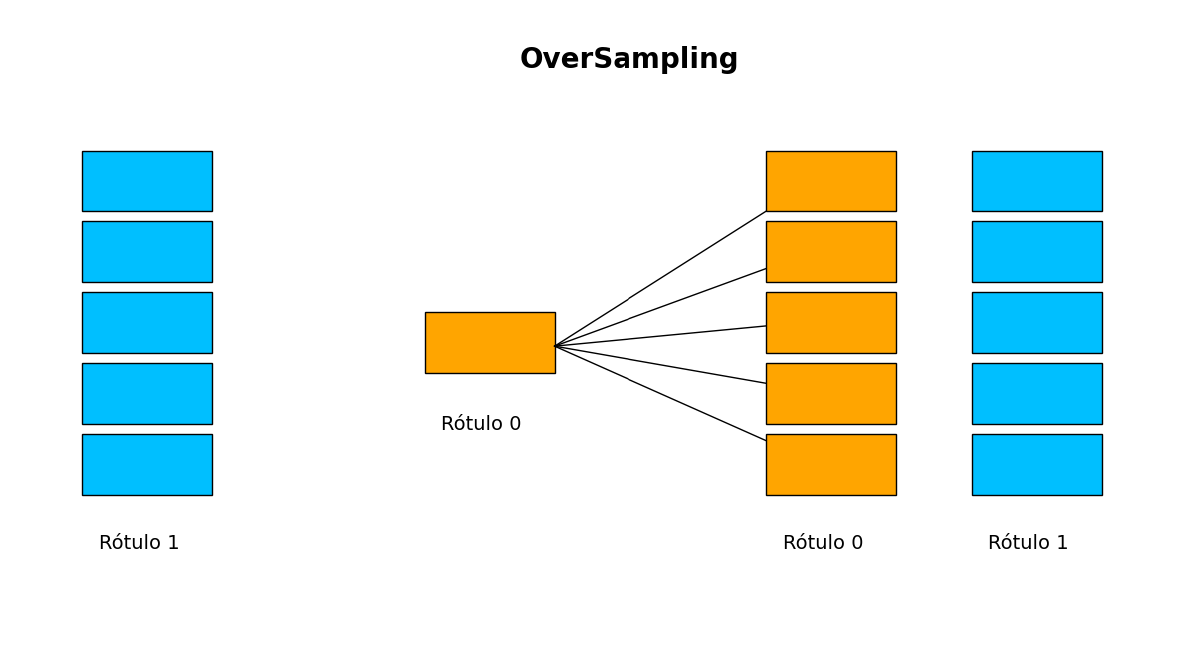
\includegraphics[width=\textwidth]{balanceamento_oversampling_silva2025.png}

      \footnotesize Sobreamostragem
    \end{column}
    \begin{column}{0.48\textwidth}
      \centering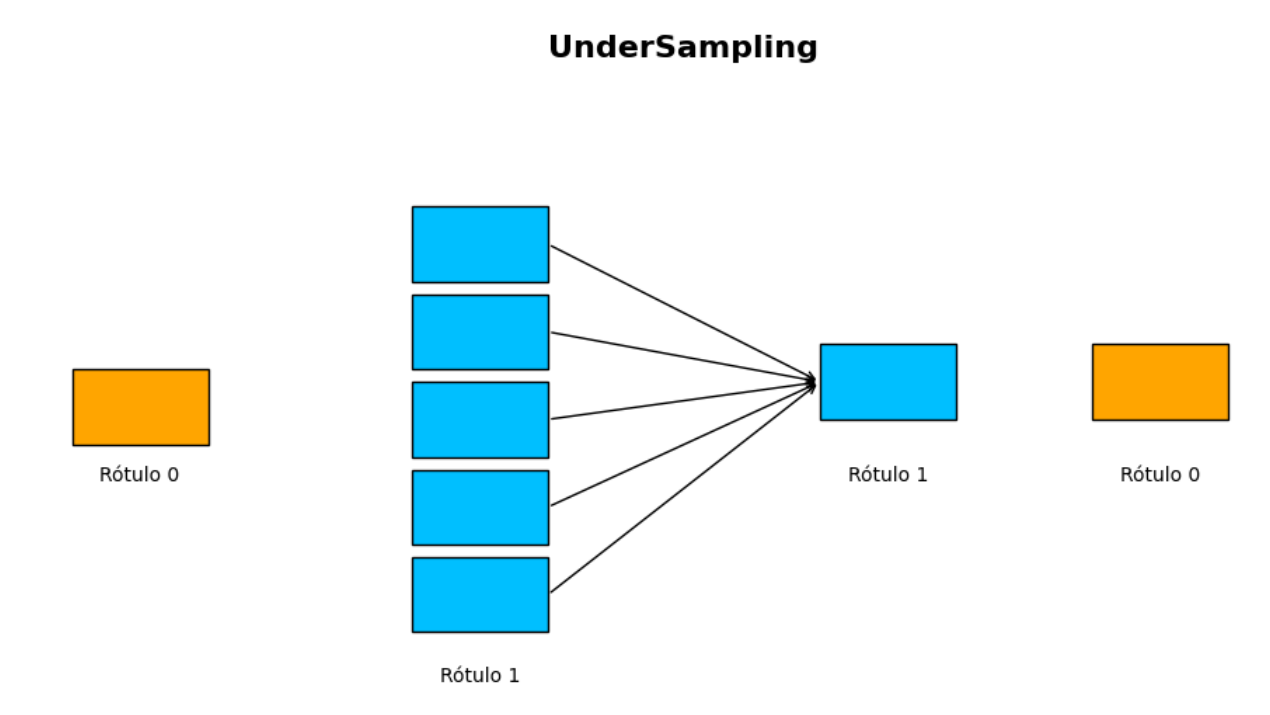
\includegraphics[width=\textwidth]{balanceamento_undersampling_silva2025.png}

      \footnotesize Subamostragem
    \end{column}
  \end{columns}
  \vspace{0.2cm}
  \begin{itemize}\small
    \item Estratégias de dados e de algoritmo (perda ponderada) discutidas na revisão
    \item Validação e teste sempre mantêm a distribuição original; avaliação por Macro-F1
  \end{itemize}
  \fonte{TCC, Seção 2.3.4; adaptado de Silva (2025).}
\end{frame}

% A2 - Convolução generalizada
\begin{frame}{Apoio A2: generalidade do operador convolucional}
  \centering
  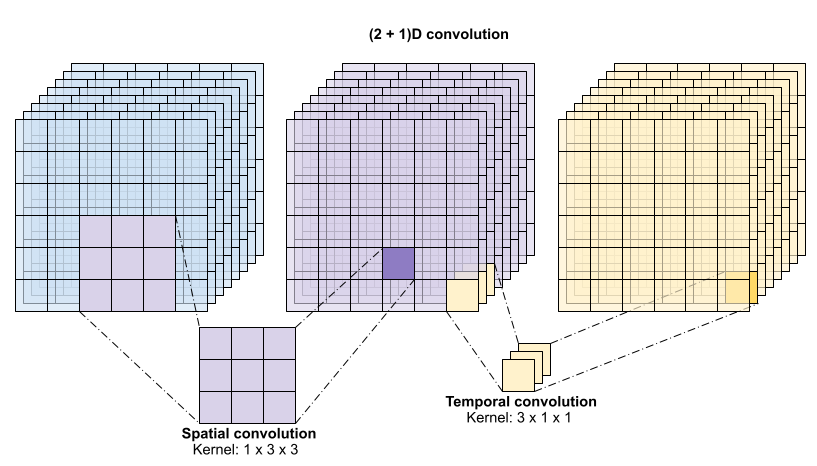
\includegraphics[width=0.52\textwidth]{2plus1CNN-converted.png}

  \small Convolução (2+1)D separa espaço e tempo; as nove bases deste trabalho são imagens estáticas 2D.
  \fonte{TCC, Seção 2.5.2.}
\end{frame}

% A3 - Riscos
\begin{frame}{Apoio A3: riscos e limitações metodológicas}
  \begin{enumerate}\small
    \item Sem emaranhamento entre os quatro subcircuitos de 5 qubits
    \item Uma semente por configuração: sem testes de significância entre inicializações
    \item \texttt{Dense20} vs. híbrido: parametrizações e não linearidades distintas, sem isolar um efeito puramente quântico
    \item Sobreposição de \textit{tracks} no GTSRB (3.990 de 5.876 imagens de teste)
    \item Restrição integral à simulação clássica, sem QPU
  \end{enumerate}
  \fonte{TCC, Seção 3.11.}
\end{frame}

% A4 - Cronograma
\begin{frame}{Apoio A4: cronograma de 16 semanas}
  \centering
  \scriptsize
  \begin{tabular}{@{}lcc@{}}
    \toprule
    \textbf{Fase} & \textbf{Semanas} & \textbf{Marco} \\
    \midrule
    1. Revisão e planejamento & 1--3 & Protocolo definido \\
    2. Inventário e preparação das 9 bases & 4--6 & Bases preparadas \\
    3. Implementação dos modelos & 7--10 & Modelos implementados \\
    4. Campanhas experimentais e auditoria & 11--14 & Resultados auditados \\
    5. Redação e finalização & 13--16 & Entrega final \\
    \bottomrule
  \end{tabular}
  \fonte{TCC, Seção 3.12 (Cronograma de trabalho).}
\end{frame}

% A5 - Siglas
\begin{frame}{Apoio A5: siglas principais}
  \scriptsize
  \begin{columns}[T]
    \begin{column}{0.48\textwidth}
      \begin{description}
        \item[CNN] Rede Neural Convolucional
        \item[PQC] Circuito Quântico Parametrizado
        \item[QML] Aprendizado de Máquina Quântico
        \item[NISQ] Computação quântica ruidosa de escala intermediária
        \item[QPU] Unidade de Processamento Quântico
      \end{description}
    \end{column}
    \begin{column}{0.48\textwidth}
      \begin{description}
        \item[IR] Razão de desbalanceamento ($n_{\max}/n_{\min}$)
        \item[CV] Coeficiente de variação
        \item[TP/FP/FN/TN] Verdadeiro/falso positivo/negativo
        \item[ROC/AUC] Curva ROC e área sob a curva
        \item[Grad-CAM] Mapeamento de ativação de classe por gradiente
      \end{description}
    \end{column}
  \end{columns}
\end{frame}

\end{document}



